\documentclass[acmsmall,screen,pdfa]{acmart}

\def\BibTeX{{\rm B\kern-.05em{\sc i\kern-.025em b}\kern-.08em
    T\kern-.1667em\lower.7ex\hbox{E}\kern-.125emX}}

\usepackage{tikz}
\usepackage[inline]{enumitem}
\usepackage{booktabs}
\usepackage{amsmath}
\usepackage{relsize}
\usepackage{cleveref}
\usepackage{multicol}
\usepackage{multirow}
\usepackage{units}
\usepackage{numprint}
\usepackage{subfigure}
\usepackage{soul}
\usepackage{array}

\usepackage{algorithm}
\usepackage[noend]{algpseudocode}

\usetikzlibrary{
    matrix,
    decorations.pathreplacing, 
    calc, 
    positioning,
    fit, 
    backgrounds, 
    shapes, 
    shapes.misc,
    patterns}



%%\acmSubmissionID{123-A56-BU3}

%%\citestyle{acmauthoryear}

% Copyright
% \setcopyright{acmcopyright}
\copyrightyear{2023}

% DOI

\setcopyright{acmlicensed}
\acmJournal{PACMMOD}
\acmYear{2023} \acmVolume{1} \acmNumber{1} \acmArticle{2} \acmMonth{5} \acmPrice{15.00}
\acmDOI{10.1145/3588682}

%Conference
% \settopmatter{printacmref=false, printccs=false, printfolios=false}

% \pagestyle{empty} % removes running headers
\keywords{Redundancy Exploitation; Lossless Compression; Linear Algebra; Machine Learning; Workload-aware Optimization; Large-scale; Declarative; Online Compression}

\begin{CCSXML}
<ccs2012>
<concept>
<concept_id>10003752.10003809.10010031.10002975</concept_id>
<concept_desc>Theory of computation~Data compression</concept_desc>
<concept_significance>500</concept_significance>
</concept>
<concept>
<concept_id>10002951.10002952.10002971.10003451.10002975</concept_id>
<concept_desc>Information systems~Data compression</concept_desc>
<concept_significance>500</concept_significance>
</concept>
<concept>
<concept_id>10010147.10010148.10010149.10010158</concept_id>
<concept_desc>Computing methodologies~Linear algebra algorithms</concept_desc>
<concept_significance>300</concept_significance>
</concept>
<concept>
<concept_id>10002951.10002952.10002971.10003450.10010828</concept_id>
<concept_desc>Information systems~Data scans</concept_desc>
<concept_significance>300</concept_significance>
</concept>
<concept>
<concept_id>10010147.10010257</concept_id>
<concept_desc>Computing methodologies~Machine learning</concept_desc>
<concept_significance>300</concept_significance>
</concept>
</ccs2012>
\end{CCSXML}

\ccsdesc[500]{Theory of computation~Data compression}
\ccsdesc[500]{Information systems~Data compression}
\ccsdesc[300]{Computing methodologies~Linear algebra algorithms}
\ccsdesc[300]{Information systems~Data scans}
\ccsdesc[300]{Computing methodologies~Machine learning}



\newcommand{\mycomment}[1]{

    \noindent \rule{\linewidth}{0.2mm}

    \noindent #1

    \noindent \rule{\linewidth}{0.2mm}}


\newcommand{\tmpFigure}[2]{
    \begin{figure}
        \includegraphics[width=\linewidth]{example-image}
        \caption{#2}
        \Description[#1]{#2}
    \end{figure}
}

\newcommand{\largeTmpFigure}[2]{
    \begin{figure*}
        \includegraphics[width=\linewidth]{example-image}
        \caption{#2}
        \Description[#1]{#2}
    \end{figure*}
}

% REMOVE ALL COMMENTS:
%\renewcommand{\mycomment}[1]{}

\newcommand{\todo}[1]{{\color{red} \mycomment{#1}}}

\newcommand{\commentBauns}[1]{{\color{blue} \mycomment{#1}}}

% Variables
\newcommand{\Gv}{\mathcal{G}}
\newcommand{\Dv}{\mathcal{D}}
\newcommand{\Tv}{\mathcal{T}}
\newcommand{\Ov}{\mathcal{O}}
\newcommand{\Rv}{\mathcal{R}}
\newcommand{\Cv}{\mathcal{C}}
\newcommand{\Sv}{\mathcal{S}}


% vertical sepereator
\newcommand{\rulesep}{\unskip\ \vrule\ }
\setlength{\textfloatsep}{9pt}

% math commands
\newcommand{\mat}[1]{\ensuremath{\mathbf{#1}}}
\newcommand{\card}[1]{\lvert #1\rvert}
\newcommand{\num}[1]{\numprint{#1}}
\npstyleenglish %. digits and , thousand seperators

% unit commands
\newcommand{\h}{\unit{\,h}}
\newcommand{\s}{\unit{\,s}}
\newcommand{\ms}{\unit{\,ms}}
\newcommand{\bbb}{\unit{\,b}}
\newcommand{\bb}{\unit{\,B}}
\newcommand{\kb}{\unit{\,KB}}
\newcommand{\mb}{\unit{\,MB}}
\newcommand{\gb}{\unit{\,GB}}
\newcommand{\tb}{\unit{\,TB}}
\newcommand{\mbs}{\unit{\,MB/s}} %{~\unitfrac{MB}{s}}
\newcommand{\gbs}{\unit{\,GB/s}} %{~\unitfrac{GB}{s}} 
\newcommand{\gflop}{\unit{\,GFLOP}} %{~\unitfrac{GFLOP}{s}}
\newcommand{\gflops}{\unit{\,GFLOP/s}} %{~\unitfrac{GFLOP}{s}}
\newcommand{\tflops}{\unit{\,TFLOP/s}} %{~\unitfrac{TFLOP}{s}}

\clubpenalty = 10000
\widowpenalty = 10000
\sloppy
\frenchspacing


\tikzset{ts/.style={text height = 0.5ex, text depth=.08ex}}

\tikzset{cg/.style={
            matrix of nodes, anchor=north,
            every node/.style={inner sep=0.5mm},
            % nodes={},
            % column 1/.style={nodes={text width=0.5cm, align=right}}
        }}
\tikzset{cgs/.style={
            matrix of nodes, anchor=north,
            every node/.style={anchor=base, ts},
            nodes={},
            % column 1/.style={nodes={text width=0.45cm, align=right}}
        }}
\tikzset{mlabel/.style={yshift=0.1cm}}
\tikzset{dictL/.style={right, align=right, xshift= 1.cm, node distance=1cm, ts}}
\tikzset{dict/.style={
    ts,    
    right,
    xshift= -1cm,
    text width=2.4ex,  node distance=1cm}}
\tikzset{bb/.style={draw, inner sep=-0.5mm, rounded corners}}


\newcommand{\name}{\textsc{\emph{Aware}}}
\newcommand{\sname}{\textsc{\emph{Sys XYC}}}

% show diff:

% \newcommand{\blue}[1]{\color{blue}  #1 \color{black}}
% \newcommand{\redd}[1]{\color{red}  \st{#1} \color{black}}
% \newcommand{\change}[1]{\color{teal} #1 \color{black}}

% disable diff:

\newcommand{\blue}[1]{\ #1}
\newcommand{\redd}[1]{}
\newcommand{\change}[1]{\ #1}



% \newcommand{\source}{../experiments/plots}
\newcommand{\source}{fig/results}

\ExplSyntaxOn
\cs_new:Npn \expandableinput #1
  { \use:c { @@input } { \file_full_name:n {#1} } }
\AddToHook{env/tabular/begin}
  { \cs_set_eq:NN \input \expandableinput }
\ExplSyntaxOff


\algnewcommand{\SLIf}[2]{\State\algorithmicif\ #1\ \algorithmicthen\  #2\ }
\algnewcommand{\SLIfnThen}[1]{\State\algorithmicif\ #1\  }
\algnewcommand{\SLThen}[1]{\State\algorithmicthen\ #1\ }
\algnewcommand{\SLElse}[1]{\State\algorithmicelse\ #1\ }




%%
%% end of the preamble, start of the body of the document source.
\begin{document}

%%
%% The "title" command has an optional parameter,
%% allowing the author to define a "short title" to be used in page headers.
% \title{AWARE: Adaptive Workload Aware Redundancy Exploitation}
\title[AWARE: Workload-aware, Redundancy-exploiting Linear Algebra]{AWARE: \\Workload-aware, Redundancy-exploiting Linear Algebra}
% \author{Paper-ID: 5}


\author{Sebastian Baunsgaard}
\orcid{0009-0001-1463-7294}
\authornote{This work was partially done at Graz University of Technology, Austria.}
\affiliation{
    \institution{Technische Universität Berlin}
    \city{Berlin}
    \country{Germany}
}

\author{Matthias Boehm}
\authornotemark[1]
\orcid{0000-0003-1344-3663}
\affiliation{
    \institution{Technische Universität Berlin}
    \city{Berlin}
    \country{Germany}
}

\renewcommand{\shortauthors}{Sebastian Baunsgaard \& Matthias Boehm}

% \keywords{}
\begin{abstract}
    \input{0_Abstract.tex}
\end{abstract}

\received{April 2022}
\received[revised]{July 2022}
\received[accepted]{August 2022}

\maketitle

% \acmBooktitle{}
% \subtitle{}


\section{Introduction}
\label{sec:Introduction}


% context: compression history and compression in ML systems
Data compression dates back to old Morse code (from the eighteen-hundreds) that uses shorter codewords for common letters~\cite{Wolfram02}.
In modern data management and machine learning (ML) systems, compression is a well-established and effective technique for fitting data in available memory, reducing I/O and memory bandwidth requirements~\cite{RamanS06, ElgoharyBHRR16}, and increasing instruction parallelism~\cite{WillhalmPBPZS09}.
Data management systems with declarative interfaces almost exclusively rely on lossless compression in order to ensure correct results,
and lightweight techniques \cite{DammeUHHL19,DammeHHL17} that offer a good balance of compression ratios and (de)compression speed.

% state-of-the-art lossy compression
\textbf{Compression:} In contrast to lossless compression in data systems, ML systems---especially for mini-batch training of deep neural networks (DNN) predominately exploit the approximate nature of ML models and apply lossy compression such as quantization (i.e., static or dynamic discretization)~\cite{tfmopt2, Zhang0KALZ17}, sparsification (clipping of low quantities)~\cite{tfmopt1, A100}, new data types (e.g., \texttt{bfloat16}, \texttt{TF32})~\cite{Saeta18, KosterWWNBCEHHK17,A100}, dimensionality reduction~\cite{IlkhechiCGMFSC20} and sampling (few step/epoch mini-batch training~\cite{SuchRLSC20}, or sampled batch training~\cite{ParkQSM19}).
However, lossy compression introduces unknown behavior on new datasets and models, which creates trust concerns and requires an exploratory trial-and-error process~\cite{WangKZAZM19}.
In contrast, lossless compression ensures result correctness, but is less commonly applied in ML.
Examples include---besides general-purpose lossless matrix compression like Snappy or LZ4---value-indexed representations~\cite{KourtisGK08, KarakasisGKGK13}, grammar-compressed matrices~\cite{TabeiSYP16}, tuple-oriented coding (TOC)~\cite{LiCZ00NP19} and Compressed Linear Algebra (CLA)~\cite{ElgoharyBHRR16, ElgoharyBHRR18}.

% background and limitations of CLA
\textbf{Redundancy Exploitation:} Sparsity exploitation is currently a major trend across the stack from hardware~\cite{A100, Olukotun21}, over systems~\cite{BoehmRHSEP18, LuoJYJ21,Sommer0ERH19}, to algorithms~\cite{tfmopt1, FrankleD0C21, abs-2107-05768}, but its applicability is limited to sparse data (many zero values). Previous work on compressed linear algebra (CLA)~\cite{ElgoharyBHRR16, ElgoharyBHRR18} further allowed for more general redundancy exploitation (with repeated values and correlation) by applying lightweight lossless compression techniques like dictionary, run-length, and offset-list encoding and executing linear algebra operations like matrix-vector multiplications and element-wise operations directly on compressed representations. CLA was integrated into Apache SystemML~\cite{BoehmDEEMPRRSST16}, but by default only applied for multi-column matrices, whose size exceed aggregated cluster memory, and all operations are supported in compressed space. These constraints ensure that online compression overheads are amortized but limit applicability in practice.

% vision
\textbf{\name~Goals and Contributions:} We aim to improve the applicability of lossless matrix compression in complex ML pipelines. The key objective is to optimize for execution time of a given workload instead of compression ratios. This metric also covers reduced compression time to amortize online compression, optimization for size if data access is the bottleneck, and fast operations via specialized compression decisions, kernels, and execution plans. To this end, we introduce a workload-aware matrix compression framework (for full matrices or tiles of a distributed matrix), and make the following detailed technical contributions:
\begin{itemize}
 \item \emph{Compression Framework:} New encodings and compressed operations (Section~\ref{sec:compression} and \ref{sec:ops}), which are designed for compressed intermediates and thus, chains of operations.
 \item \emph{Workload-aware Compression:} Novel workload-aware compression planning and compilation techniques (Section~\ref{sec:workload}).
 \item \emph{Experiments:} Local \& distributed experiments comparing uncompressed linear algebra (ULA), CLA~\cite{ElgoharyBHRR16, ElgoharyBHRR18}, TensorFlow, and \name\ on various workloads (Section~\ref{sec:Experiments}).
\end{itemize}
 

\section{Background and Overview}
\label{sec:background}

This section reviews the main characteristics of CLA
and its limitations, which directly motivate key design decisions of \name.
% Inspired by database compression schemes and sparse matrix representations,
CLA~\cite{ElgoharyBHRR16, ElgoharyBHRR18} is a lossless compression framework leveraging
column-wise compression, column co-coding (encode groups of columns as single units), and heterogeneous column encoding schemes.
This design exploits characteristics of feature matrices---with categorical and numerical features in columns---namely,
tall and skinny matrices, non-uniform sparsity, low cardinality and correlations.
Since the selection of column groups is strongly data-dependent,
CLA introduced a sampling-based compression planning for online compression after
an initial read of an input matrix.
Once compressed, specialized kernels work directly on the compressed representation if applicable and efficient,
otherwise fall back to decompression followed by uncompressed kernels.

\subsection{Limitations of CLA}


Despite CLA's compelling properties---allowing operations directly on the compressed representations---there are limitations and missing functionality that hinder general applicability.

\textbf{Compression Costs:}
The original CLA's \cite{ElgoharyBHRR16} sampling-based compression planning used a sample fraction and a co-coding algorithm
that---ignoring greedy partitioning---required $\mathcal{O}(m^3)$ group extractions from the sample.
The refined CLA \cite{ElgoharyBHRR18} %\redd{increased the sample fraction to $f=0.05$ for better robustness, but}
improved the co-coding approach via memoization to $\mathcal{O}(m^2)$ group extractions.
However, despite column classification into compressible and incompressible columns,
matrices with no or minor compression benefits were recognized much too late,
after incurring already substantial overhead.
Furthermore, the super-linear co-coding complexity becomes infeasible for millions of columns.

\textbf{Compressed Intermediates:}
CLA performs online compression for input matrices and keeps outputs of amenable operations like matrix-scalar element-wise multiplications,
or scaling and shifting compressed.
Other operations produce uncompressed outputs (e.g., after feature transformations or data cleaning).
In complex, exploratory ML pipelines there are multiple sources of redundancy though,
which would largely benefit from a more fine-grained selection of intermediates and optimization of their individual compression schemes.

\textbf{Optimization Objective:}
The design and implementation of CLA aimed at the sweet spot of compressed operation performance close to uncompressed (low in-memory overhead),
while achieving good compression ratios (fit larger data in memory, reduced I/O for large data).
Besides this hand-crafted tuning, the internal objective for selecting compression schemes and co-coding then only focuses on minimizing compressed size.
Fundamentally, however, the overall optimization objective should be total execution time,
factoring in compression, compressed operations, and potential I/O in order to better adapt to data, operation, and cluster characteristics.



% CLA
% DDC, OLE, RLE, UC. Encodings: DDC 2, OLE 1, RLE 1, UC 1. -> 4(5)

% NEW:
% DDC 4, CON 2, OLE, RLE, UC, SDC 4 * 2 * 4, PFOR 2 * 4 = 4 + 2 + 1 + 1 + 1 + 32 + 8 = ColumnGroup Index Structures 49
% Dictionary encodings: 3 (Double Dense, MatrixBlock Dense, MatrixBlock Sparse) * 49 = 147 possibilities.
% with UByte (debatable)
% DDC 5, CON 2, OLE, RLE, UC, SDC 5 * 2 * 4, PFOR 2 * 5 = 5 + 2 + 1 + 1 + 1 + 35 + 10 = ColumnGroup Index Structures 55
% Dictionary encodings: 3 (Double Dense, MatrixBlock Dense, MatrixBlock Sparse) * 55 = 165 possibilities.

% DDC 7 * 2*( FOR), CON 2, UC, SDC 7 * 4 * 3 (Zero,_, FOR)  SDCSingle, 4*2 
% 7 *2 + 2 + 1 + 1 + 1 + 7*4*3 + 4*2 = 109 col group index structures.
%  3 * 111 = 333

% YetAgain:
% DT = 3 // dictionary types
% DDC 7 * DT  = 21
% DDCFOR 7 * DT =21
% CON  DT = 3
% Empty 1  = 1
% Uncompressed = 2 // Sparse or dense 
% SDC 7 * 4 * DT = 84
% SDC Zero 7 * 4 * DT = 84
% SDC Single 4 * DT = 12
% SDC Single Zero 4 * DT = 12
% SDC FOR 7 * 4 * DT = 84
% RLE DT = 3
%% Sum = 327

\begin{table}[!t]
    \centering \setlength\tabcolsep{10pt}
    \caption{\label{tab:diff}Differences of CLA and \name}
    \vspace{-0.4cm}
    \begin{tabular}{rcc}
        \toprule
                               & \textbf{CLA}~\cite{ElgoharyBHRR16,ElgoharyBHRR18} & \textbf{\name}   \\
        \midrule
        Co-Coding              & $\mathcal{O}(m^2)$                                & $\mathcal{O}(m)$ \\
        Column Group Encodings & 4 (5)                                             & 7 (327)          \\
        Materialization        & Eager                                             & Deferred         \\
        Optimization Objective & Data                                              & Data \& Ops      \\
        Matrix Multiplication  & MV, VM                                            & MV, VM, MM       \\

        \bottomrule
    \end{tabular}
    \vspace{0.3cm}
\end{table}


\subsection{\name\ Overview}

Our workload-aware compression addresses these limitations with new techniques for compression planning, compressed intermediates, and different optimization objectives. Table~\ref{tab:diff} highlights these key differences between CLA and \name.
%
First, to reduce compression time, we introduce a new co-coding technique that performs group \emph{combinations} instead of group \emph{extractions}, reducing the overhead to analyze groups. Our co-coding approach further includes a new enumeration heuristic that only evaluates $\mathcal{O}(m)$ group combinations.
%
Second, for extended utilization of compressed intermediates, we provide new column group encodings that facilitate shallow-copy operations. Table~\ref{tab:diff} shows the number of high-level column group types and---in parenthesis---the total number of variations of these encodings. We also introduce a deferred operation/encoding design, where compressed operations can output different types of encodings, allowing compressed intermediates where CLA would decompress or return inefficient representations. Furthermore, \name\ natively supports compressed matrix-matrix multiplication (even with two compressed inputs), unlike CLA that would process it via repeated matrix-vector multiplications and thus decompresses one side.
%
And above all, \name\ uses a cost-based optimization objective of minimizing the workload execution time and thus, tuning the compression process, the compressed representation, and compressed operations in a principled way.


\section{Compression}
\label{sec:compression}

This section describes \name's compressed representation, selected new concepts, and the overall compression algorithm.
The new encoding schemes are designed for redundancy exploitation across operations, while the new compression algorithm ensures fast, easy to amortize compression.

\subsection{Compressed Representation}
\label{sec:compressedRepresentation}


\begin{table}[!t]
    \centering \setlength\tabcolsep{10pt}
    \caption{\label{tab:colgroups}Overview of CLA and \name \ Column Groups.}
    \vspace{-0.4cm}
    \begin{tabular}{llcc}
        \toprule
        \textbf{Type} & \textbf{Description}      & \textbf{CLA}~\cite{ElgoharyBHRR16,ElgoharyBHRR18} & \textbf{\name} \\
        \midrule
        CON           & Constant or Empty Columns &                                                   & \checkmark     \\
        DDC           & Dense Dictionary Coding   & \checkmark                                        & \checkmark     \\
        OLE           & Offset-list Encoding      & \checkmark                                        & (\checkmark)   \\
        FOR           & Frame of Reference        &                                                   & \checkmark     \\
        RLE           & Run-length Encoding       & \checkmark                                        & (\checkmark)   \\
        SDC           & Sparse Dictionary Coding  &                                                   & \checkmark     \\
        UC            & Uncompressed (dense/sparse) & \checkmark                                        & \checkmark     \\
        \bottomrule
    \end{tabular}
    \vspace{0.1cm}
\end{table}


% with the ``best'' encoding type, by some objective.
% Our optimizers minimize compression size, workload cost or hybrid costs combining multiple objectives.

\name\ encodes each column group independently in a specific encoding type.
Table~\ref{tab:colgroups} shows these column-group encodings, as well as the differences to CLA.
Figure~\ref{fig:encoded} then presents an example of compressing a $10\times 6$ matrix into three single-column groups (0, 2 and 5), one two-column group ($\{1,3\}$), and an empty group. Also shown is an element-wise scalar subtraction on the compressed matrix, creating two alternative compressed outputs (A and B).


\textbf{Dense Dictionary Coding (DDC)} contains two parts: a \emph{dictionary} with the distinct value tuples in the column group,
(shown in Figure~\ref{fig:encoded} as a Dict with 2 values for column $\{0\}$), and an \emph{index structure} with a row-to-tuple mapping (e.g., dictionary position). DDC is dense because each row input is assigned a code in the map.

\textbf{Sparse Dictionary Coding (SDC)}
is a combination of DDC and sparse matrix formats like compressed sparse rows (CSR).
An example is shown in yellow for columns $\{1,3\}$ in Figure~\ref{fig:encoded}. Like DDC, each group has a dictionary of all unique tuples except the most frequent tuple named ``Def'' for default. This scheme encodes row locations of non-default tuples in the index structure as row-index pairs. This approach is similar to compressed sparse columns (CSC) that store row-index/value pairs for non-zero values, but extends it for general redundancy exploitation (default values, dictionary references).
% SDC Index structure
The row part is further specialized to delta offsets (``Off'') from previous rows to allow smaller physical codewords.
Finally, a ``Map'' (index part of CSC) maps offsets to tuples in the dictionary, similar to DDC.
% Specialization
SDC specializes into SDCZero, where zero default entries are removed like in the
$\{2\}$
blue column group, and SDCSingle for binary data (one dictionary entry, one default), removing the need of codes like in the
$\{4\}$
orange column group.

\textbf{Frame of Reference (FOR)} is used as a second layer on top of DDC or SDC (called DDCFOR, SDCFOR). This encoding shallow-copies the index structures and dictionaries, and allocates a reference tuple, that indicates a global value offset.
An SDC group can zero-out the default tuple by adding it to the dictionary and subtracting it from the reference tuple (converted to SDCZero).

\textbf{Offset-list Encoding (OLE)} is a CLA encoding scheme, but largely superseded by SDC. SDC has in general worse compression than OLE, but SDC allow the group to densify its values without having to modify its index structure, while if densified OLE encode a value for each row making it inefficient and potentially bigger.

\textbf{Run-length Encoding (RLE)} is unlikely beneficial in \name\ since co-coding many columns---which is good for operation performance, and likely to be done in scenarios with good RLE compression---makes it unlikely to retain sufficiently long runs. RLE also reallocates the index structure on densifying operations.

\textbf{Constant Encodings} are used for empty, constant columns, and constant tuple column groups. CLA encodes such groups using run-length encoding (RLE).
Instead we specialize with constant groups in order to simplify operations with compressed outputs.

\textbf{Dictionaries:} CLA uses basic \texttt{FP64} dictionaries. In contrast, \name \ generalizes the data binding of dictionaries and uses basic \texttt{FP64} and \texttt{INT8} arrays, or sparse matrices.
The more columns co-coded, the more zeros might be included in unique tuples and thus, warrant a sparse dictionary. \name \ does not share dictionaries across multiple column groups like CLA does in some cases.

\textbf{Index Encodings:} The different column group implementations share common primitives such as Map and Off, of different value types (not shown in the figure). Map supports encodings in Bit, Byte, UByte, Char, Char+Byte and Int, while Off supports delta-encoded Byte or Char arrays, and specializations for one/two offsets.

\textbf{Overlapping Column Groups:} \name\ allows column groups to overlap with partial sum semantics. Multiple column groups may refer to the same column but store separate dictionaries and index structures. Overlapping helps column groups preserve (and due to compression, eliminate) structural redundancy of intermediates for chains of operations such as matrix multiplication, row sums aggregation, and scalar or column addition.



\def\bottom#1#2{\hbox{\vbox to #1{\vfill\hbox{#2}}}}
\begin{figure*}
    \centering
    \resizebox{\textwidth}{!}
    {
    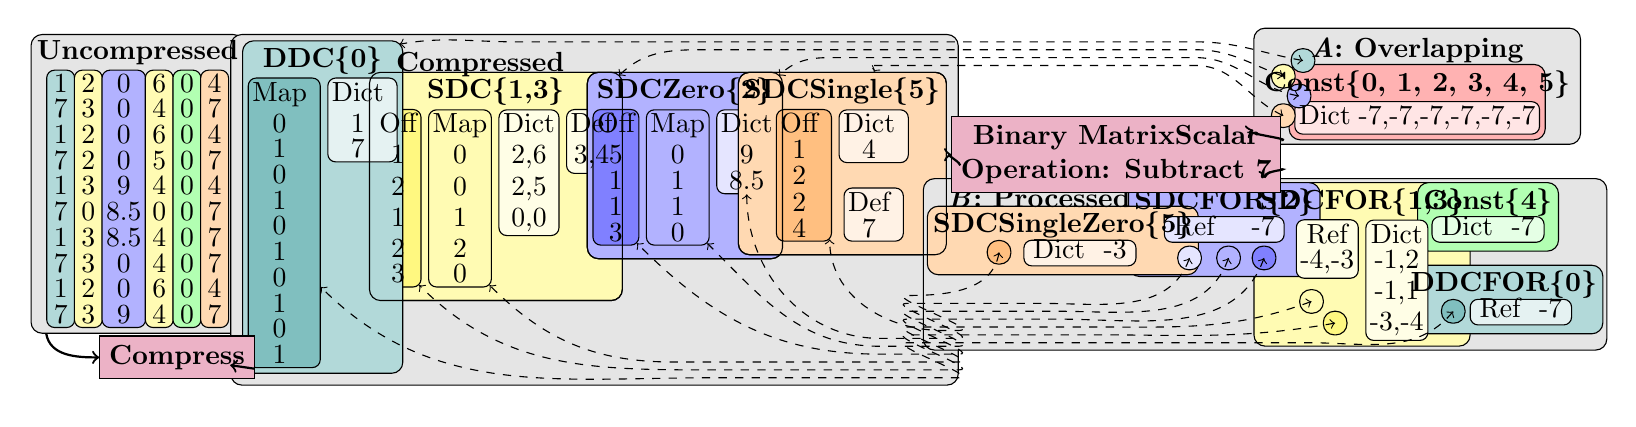
\begin{tikzpicture}[font=\Small, ampersand replacement=\&]

        \begin{scope}[xshift=-0.35cm]
            \matrix[cg, every node/.style={minimum width=1em,inner sep=0.5mm},
            ](UC) at(-0.2cm,0.5) {
                1 \& 2 \& 0   \& 6 \& 0 \& 4 \\
                7 \& 3 \& 0   \& 4 \& 0 \& 7 \\
                1 \& 2 \& 0   \& 6 \& 0 \& 4 \\
                7 \& 2 \& 0   \& 5 \& 0 \& 7 \\
                1 \& 3 \& 9   \& 4 \& 0 \& 4 \\
                7 \& 0 \& 8.5 \& 0 \& 0 \& 7 \\
                1 \& 3 \& 8.5 \& 4 \& 0 \& 7 \\
                7 \& 3 \& 0   \& 4 \& 0 \& 7 \\
                1 \& 2 \& 0   \& 6 \& 0 \& 4 \\
                7 \& 3 \& 9   \& 4 \& 0 \& 7 \\
            };
            \node[mlabel](UCL) at (UC.north){\textbf{Uncompressed}};
            \begin{scope}[on background layer]
                \node[bb, fit=(UCL) (UC), fill = black!10](UCBB){};
                \node[bb, thin,fit=(UC-1-1) (UC-10-1),          inner sep = -0.15, rounded corners=1mm, fill = teal!30]{};
                \node[bb, thin,fit=(UC-1-2) (UC-10-2),          inner sep = -0.15, rounded corners=1mm, fill = yellow!30]{};
                \node[bb, thin,fit=(UC-1-3) (UC-10-3) (UC-6-3), inner sep = -0.15, rounded corners=1mm, fill = blue!30]  {};
                \node[bb, thin,fit=(UC-1-4) (UC-10-4),          inner sep = -0.15, rounded corners=1mm, fill = yellow!30]{};
                \node[bb, thin,fit=(UC-1-5) (UC-10-5),          inner sep = -0.15, rounded corners=1mm, fill = green!30] {};
                \node[bb, thin,fit=(UC-1-6) (UC-10-6),          inner sep = -0.15, rounded corners=1mm, fill = orange!30]{};
            \end{scope}
        \end{scope}

        \begin{scope}[xshift=0.8cm]
            % G1 SDC:
            \matrix[cg](G1) at (3.2,0) {
                Off \& [1mm] Map \& [1mm] Dict \& [1mm] Def \\
                1   \& 0                                          \& 2,6                                         \& 3,4                                        \\
                2   \& 0                                          \& 2,5                                         \&                                            \\
                1   \& 1                                          \& 0,0                                         \&                                            \\
                2   \& 2                                          \&                                             \&                                            \\
                3   \& 0                                          \&                                             \&                                            \\
                \   \&                                            \&                                             \&                                            \\
            };

            \node[mlabel](G1L) at (G1.north){\textbf{SDC\{1,3\}}};
            \node[bb, fit=(G1L.north) (G1.south) (G1.east) (G1.west)](G1BG){};

            % G2 SDCZero:              
            \matrix[cg](G2) at (5.6,0){
                Off \& [1mm] Map \& [1mm] Dict \\
                5   \& 0                                          \& 9                                           \\
                1   \& 1                                          \& 8.5                                         \\
                1   \& 1                                          \&                                             \\
                3   \& 0                                          \&                                             \\
                \   \&                                            \&                                             \\
            };
            \node[mlabel](G2L) at (G2.north){\textbf{SDCZero\{2\}}};
            \node[bb, fit=(G2L.north) (G2.south) (G2.east) (G2.west)](G2BG){};

            % G4 SDCSingle:
            \matrix[cg, align=center ](G4) at(7.6,0){
                Off \& [1mm] Dict \\
                1   \& 4                                           \\
                2   \&                                             \\
                2   \& Def                                         \\
                4   \& 7                                           \\
                \   \&                                             \\
            };
            \node[mlabel](G4L) at (G4.north){\textbf{SDCSingle\{5\}}};
            \node[bb, fit=(G4L) (G4)](G4BG){};
            \node[mlabel](COMPL) at ([yshift=0.35cm, xshift=-0.2cm]G1.north){\textbf{Compressed}};


            % G5 DDC:
            \matrix[cg, align=center](G5) at(1,0.4){
                Map \& [1mm] Dict \\
                0   \& 1                                           \\
                1   \& 7                                           \\
                0   \&                                             \\
                1   \&                                             \\
                0   \&                                             \\
                1   \&                                             \\
                0   \&                                             \\
                1   \&                                             \\
                0   \&                                             \\
                1   \&                                             \\
            };

            \node[mlabel](G5L) at (G5.north){\textbf{DDC\{0\}}};

            \begin{scope}[on background layer]
                \node[bb, inner sep=1mm, fit=(G4L) (G1) (G2)  (G4) (G5) (COMPL) , fill=black!10](COMPBB){};
                \node[bb, fit=(G1L) (G1), fill=yellow!30](G1BB){};
                \node[bb, thin,fit=(G1-1-1) (G1-6-1), inner sep = -0.15, rounded corners=1mm, fill = yellow!50](G1Off){};
                \node[bb, thin,fit=(G1-1-2) (G1-6-2), inner sep = -0.15, rounded corners=1mm, fill = yellow!30](G1Map){};
                \node[bb, thin,fit=(G1-1-3) (G1-4-3), inner sep = -0.15, rounded corners=1mm, fill = yellow!10](G1Dic){};
                \node[bb, thin,fit=(G1-1-4) (G1-2-4), inner sep = -0.15, rounded corners=1mm, fill = yellow!10](G1Def){};

                \node[bb, fit=(G2L) (G2), fill=blue!30](G2BB){};
                \node[bb, thin,fit=(G2-1-1) (G2-5-1), inner sep = -0.15, rounded corners=1mm, fill=blue!50](G2Off){};
                \node[bb, thin,fit=(G2-1-2) (G2-5-2), inner sep = -0.15, rounded corners=1mm, fill=blue!30](G2Map){};
                \node[bb, thin,fit=(G2-1-3) (G2-3-3), inner sep = -0.15, rounded corners=1mm, fill=blue!10](G2Dic){};

                % \node[bb, fit=(G3L) (G3), fill=green!30](G3BB){};

                \node[bb, fit=(G4L) (G4), fill=orange!30](G4BB){};
                \node[bb, thin,fit=(G4-1-1) (G4-5-1), inner sep = -0.15, rounded corners=1mm, fill=orange!50](G4Off){};
                \node[bb, thin,fit=(G4-1-2) (G4-2-2), inner sep = -0.15, rounded corners=1mm, fill=orange!10](G4Dic){};
                \node[bb, thin,fit=(G4-4-2) (G4-5-2), inner sep = -0.15, rounded corners=1mm, fill=orange!10](G4Def){};

                \node[bb, fit=(G5L) (G5), fill=teal!30](G5BB){};
                \node[bb, thin,fit=(G5-1-1) (G5-11-1), inner sep = -0.15, rounded corners=1mm, fill=teal!50](G5Map){};
                \node[bb, thin,fit=(G5-1-2) (G5-3-2), inner sep = -0.15, rounded corners=1mm, fill=teal!10](G5Dic){};
            \end{scope}



        \end{scope}

        \begin{scope}[yshift=0.4cm]
            \begin{scope}[xshift=14.cm, yshift=-0.5cm]
                % G1 SDCZero:
                \begin{scope}[yshift=0.25cm]
                    \node[bb, inner sep=1.5mm, outer sep=1mm, fill=teal!30, rectangle] (GDDCA) at (0.25,0.35)  { };
                    \node[bb, inner sep=1.5mm, outer sep=1mm, fill=yellow!30, rectangle] (G1A) at (0,0.15){ };
                    \node[bb, inner sep=1.5mm, outer sep=1mm, fill=blue!30,   rectangle] (G2A) at (0.2,-0.1){ };
                    \node[bb, inner sep=1.5mm, outer sep=1mm, fill=orange!30, rectangle] (G4A) at (0,-0.35){ };
                \end{scope}

                \node[cg](G5A) at (1.7,0.2) {
                    Dict \& -7,-7,-7,-7,-7,-7 \\
                };
                \node[mlabel](G5AL) at (G5A.north){\textbf{Const\{0, 1, 2, 3, 4, 5\}}};
                \node[ inner sep=0mm, fit=(G1A) (G2A) (G4A) (G5AL) (G5A) ](optA){};
                \node[mlabel](optAL) at ([yshift=0.03cm]G5AL.north){\textbf{\emph{A}: Overlapping}};

                \begin{scope}[on background layer]
                    \node[bb, inner sep=0mm, fit=(optA) (optAL), fill=black!10](optA){};
                    \node[bb, fit=(G5AL.north) (G5A.south) (G5A.east) (G5A.west), fill=red!30]{};
                    \node[bb, thin, fit=(G5A-1-1) (G5A-1-2), inner sep = -0.15, rounded corners=1mm, fill = red!10](G1Dic){};
                \end{scope}

                \draw[<->, dashed] (GDDCA.center) to[out=170, in=0] ([yshift=-0.1cm, xshift=3cm]COMPBB.north east) -- ([yshift=-0.1cm]COMPBB.north east) -- ([yshift=-0.1cm, xshift=-1cm]COMPBB.north)  to [out=180, in = 10] ([yshift=-0.05cm, xshift=-0.05cm]G5BB.north east);
                \draw[<->, dashed] (G1A.center) to[out=160, in=0]   ([yshift=-0.2cm, xshift=3cm]COMPBB.north east) -- ([yshift=-0.2cm]COMPBB.north east) -- ([yshift=-0.2cm, xshift=1.5cm]COMPBB.north) to [out=180, in = 45] ([yshift=-0.05cm, xshift=-0.05cm]G1BB.north east);
                \draw[<->, dashed] (G2A.center) to[out=170, in=0]   ([yshift=-0.3cm, xshift=3cm]COMPBB.north east) -- ([yshift=-0.3cm]COMPBB.north east) -- ([yshift=-0.3cm, xshift=3cm]COMPBB.north) to [out=180, in = 45] ([yshift=-0.05cm, xshift=-0.05cm]G2BB.north east);
                \draw[<->, dashed] (G4A.center) to[out=155, in=0]   ([yshift=-0.4cm, xshift=3cm]COMPBB.north east) -- ([yshift=-0.4cm]COMPBB.north east) -- ([yshift=-0.4cm, xshift=3.5cm]COMPBB.north) to [out=180, in = 60] ([ xshift=0.4cm]G4BB.north);
                % \node at([yshift=0.1cm, xshift= 0.15cm]COMPBB.north east) {\tiny Pointers};
            \end{scope}

            \begin{scope}[xshift=15.cm, yshift=-1.8cm](optB)

                \matrix[cg](G1A2){
                    Ref   \& [1mm] Dict \\
                    -4,-3 \& -1,2                                        \\
                    \     \& -1,1                                        \\
                    \     \& -3,-4                                       \\
                };

                \node[bb, inner sep=1.5mm, outer sep=1mm, fill=yellow!30, rectangle](G1A2Map) at ([yshift = -0.02cm, xshift = -0.2cm]G1A2-3-1) {};
                \node[bb, inner sep=1.5mm, outer sep=1mm, fill=yellow!50, rectangle](G1A2Off) at ([yshift = 0.1cm, xshift = 0.1cm]G1A2-4-1) {};

                \node[mlabel](G1A2L) at (G1A2.north){\textbf{SDCFOR\{1,3\}}};

                \matrix[cgs](G2A2) at (-1.75,0){
                    Ref \&    \& -7 \\
                    \   \& \  \& \  \\
                };
                \node[bb, inner sep=1.5mm, outer sep=1mm, fill=blue!50, rectangle](G2A2Off) at ([yshift = -0.0cm, xshift= 0.01cm]G2A2-2-3) {};
                \node[bb, inner sep=1.5mm, outer sep=1mm, fill=blue!30, rectangle](G2A2Map) at ([yshift = -0.0cm, xshift= -0.06cm]G2A2-2-2) {};
                \node[bb, inner sep=1.5mm, outer sep=1mm, fill=blue!10, rectangle](G2A2Dic) at ([yshift = -0.0cm, xshift= -0.06cm]G2A2-2-1) {};
                \node[mlabel](G2A2L) at (G2A2.north){\textbf{SDCFOR\{2\}}};



                \matrix[cgs](G4A2) at(-3.8,-0.3){
                    \  \& [2mm]  Dict \& -3 \\
                };
                \node[bb, inner sep=1.5mm, outer sep=1mm, fill=orange!50, rectangle](G4A2Off) at ([yshift = 0.05cm]G4A2-1-1) {};

                \node[mlabel](G4A2L) at (G4A2.north){\textbf{SDCSingleZero\{5\}}};

                \matrix[cgs](G3A2) at(1.60, 0){
                    Dict \& -7 \\
                };
                \node[mlabel](G3A2L) at (G3A2.north){\textbf{Const\{4\}}};

                \matrix[cgs](G5A2) at(1.80,-1.05){
                    \  \& [2mm] Ref \& -7 \\
                };
                \node[bb, inner sep=1.5mm, outer sep=1mm, fill=teal!50, rectangle](G5A2Map) at ([yshift = 0.05cm, xshift=0.1cm]G5A2-1-1) {};
                \node[mlabel](G5A2L) at (G5A2.north){\textbf{DDCFOR\{0\}}};

                \node[mlabel](optAL) at ([yshift=0.35cm, xshift = -0.3cm]G4A2.north){\textbf{\emph{B}: Processed}};

                \begin{scope}[on background layer]
                    \node[bb, inner sep=0mm, fit=(G1A2L) (G1A2) (G2A2L) (G2A2) (G3A2) (G3A2L) (G4A2) (G4A2L) (G5A2) (G5A2L), fill=black!10](optB){};
                    \node[bb, fit=(G1A2L) (G1A2), fill=yellow!30](G1ABB){};
                    \node[bb, fit=(G2A2L) (G2A2), fill=blue!30](G2ABB){};
                    \node[bb, fit=(G3A2L) (G3A2), fill=green!30]{};
                    \node[bb, fit=(G4A2L) (G4A2), fill=orange!30]{};
                    \node[bb, fit=(G5A2L) (G5A2), fill=teal!30]{};
                    \node[bb, thin,fit=(G1A2-1-1) (G1A2-2-1), inner sep = -0.15, rounded corners=1mm, fill = yellow!10](){};
                    \node[bb, thin,fit=(G1A2-1-2) (G1A2-4-2), inner sep = -0.15, rounded corners=1mm, fill = yellow!10](){};


                    \node[bb, thin,fit=(G2A2-1-1) (G2A2-1-3), inner sep = -0.15, rounded corners=1mm, fill = blue!10, yshift=0.4mm](){};
                    \node[bb, thin,fit=(G3A2-1-1) (G3A2-1-2), inner sep = -0.15, rounded corners=1mm, fill = green!10, yshift=0.4mm](){};
                    \node[bb, thin,fit=(G5A2-1-2) (G5A2-1-3), inner sep = -0.15, rounded corners=1mm, fill = teal!10, yshift=0.4mm](){};
                    \node[bb, thin,fit=(G4A2-1-2) (G4A2-1-3), inner sep = -0.15, rounded corners=1mm, fill = orange!10, yshift=0.4mm](){};
                \end{scope}

                %% from bottom
                \draw[<->, dashed] (G5A2Map.center)
                to[out=-130, in=0] ([yshift=0.1cm, xshift = 4.9cm]optB.south west)
                to[out=-180, in=0] ([yshift=0.1cm, xshift = -0.2cm]optB.south west)
                to[out=-180, in=0] ([yshift=0.1cm]COMPBB.south east)
                to[out =180, in = 0] ([yshift=0.1cm, xshift= 1.5cm]COMPBB.south)
                to[ out=180, in = -45] ([xshift=-0.0cm, yshift=1.03cm]G5Map.south east);

                \draw[<->, dashed] (G1A2Off.center)
                to[out=-170, in=0] ([yshift=0.2cm, xshift = 2.2cm]optB.south west)
                to[out=-180, in=0] ([yshift=0.2cm, xshift = -0.2cm]optB.south west)
                to[out=-180, in=0] ([yshift=0.2cm]COMPBB.south east)
                to[out =180, in = 0] ([yshift=0.2cm, xshift= 1.5cm]COMPBB.south)
                to[ out=180, in = -45] ([xshift=-0.03cm, yshift=0.03cm]G1Off.south east);

                \draw[<->, dashed] (G1A2Map.center)
                to[out=-160, in=0] ([yshift=0.3cm, xshift = 2.2cm]optB.south west)
                to[out=-180, in=0] ([yshift=0.3cm, xshift = -0.2cm]optB.south west)
                to[out=-180, in=0] ([yshift=0.3cm] COMPBB.south east)
                to[out =180, in = 0] ([yshift=0.3cm, xshift= 1cm]COMPBB.south)
                to[ out=180, in = -45] ([xshift=-0.03cm, yshift=0.03cm]G1Map.south east);


                \draw[<->, dashed] (G2A2Off.center)
                to[out=-110, in=0] ([yshift=0.4cm, xshift = 1.7cm]optB.south west)
                to[out=-180, in=0] ([yshift=0.4cm, xshift = -0.2cm]optB.south west)
                to[out=-180, in=0] ([yshift=0.4cm]COMPBB.south east)
                to[out =180, in = 0] ([yshift=0.4cm, xshift= -1cm]COMPBB.south east)
                to[ out=180, in = -45] ([xshift=-0.03cm, yshift=0.03cm]G2Off.south east);

                \draw[<->, dashed] (G2A2Map.center)
                to[out=-110, in=0] ([yshift=0.5cm, xshift = 1.7cm]optB.south west)
                to[out=-180, in=0] ([yshift=0.5cm, xshift = -0.2cm]optB.south west)
                to[out=-180, in=0] ([yshift=0.5cm]COMPBB.south east)
                to[out =180, in = 0] ([yshift=0.5cm, xshift= -1cm]COMPBB.south east)
                to[ out=180, in = -45] ([xshift=-0.03cm, yshift=0.03cm]G2Map.south east);


                \draw[<->, dashed] (G2A2Dic.center)
                to[out=-110, in=0] ([yshift=0.6cm, xshift = 1.5cm]optB.south west)
                to[out=-180, in=0] ([yshift=0.6cm, xshift = -0.2cm]optB.south west)
                to[out=-180, in=0] ([yshift=0.6cm]COMPBB.south east)
                to[out =180, in = 0] ([yshift=0.6cm, xshift= -1cm]COMPBB.south east)
                to[ out=180, in = -90] (G2Dic.south);

                \draw[<->, dashed] (G4A2Off.center)
                to[out=-100, in=0] ([yshift=0.7cm, xshift = -0.2cm]optB.south west)
                to[out=-180, in=0] ([yshift=0.7cm]COMPBB.south east)
                to[out =180, in = 0] ([yshift=0.7cm, xshift= -0.2cm]COMPBB.south east)
                to[ out=180, in = 270] ([xshift=-0.03cm, yshift=0.03cm]G4Off.south east);


            \end{scope}
        \end{scope}

        \node[align = center, draw, fill = purple!30](compressIns) at ([xshift=0.5cm, yshift=-0.3cm] UCBB.south) {\textbf{Compress}};
        \draw[->, thick] ([xshift=0.2cm]UCBB.south west) to[out=-80 , in =180] (compressIns.west);
        \draw[->, thick] (compressIns) to ([yshift=0.26cm]COMPBB.south west);


        \node[align = center, draw, fill = purple!30](sup7) at ([xshift=2.0cm, yshift=0.7cm] COMPBB.east) {\textbf{Binary MatrixScalar}\\\textbf{Operation: Subtract 7}};

        \draw[->, thick] (COMPBB) to[ out=7 , in =180] (sup7);
        \draw[->, thick] (sup7) to[ out=5 , in =195] (optA);
        \draw[->, thick] (sup7) to[ out=-5 , in =90] (optB);

    \end{tikzpicture}
    }
    \vspace{-0.65cm}
    \caption{\label{fig:encoded}Example \name \ Matrix Compression and Operation {\normalfont(with Alternative Compressed Outputs)}.}
    \Description[Example \name \ Matrix Compression and Operation]{}
\end{figure*}

\textbf{An Operation Example:}
Figure~\ref{fig:encoded} (right) shows an operation example subtracting 7 from the compressed matrix.
Option \emph{A} creates an overlapping representation with pointers to the input column groups and a new constant group subtracting 7 from the entire matrix.
In contrast, Option \emph{B} performs the subtraction on all column groups, creating different output group types.
The empty column becomes a \emph{Const} group of -7.
Column $\{2\}$ in blue becomes a \emph{SDCFOR} group that copies pointers to the previous dictionary and index structure, and only materializes a new reference value.
The \emph{SDCSingle} group in orange becomes an \emph{SDCSingleZero} because Def 7-7 yields 0.
The \emph{SDC} group in yellow has a different default value, and thus, produces an \emph{SDCFOR} group, where we subtract the default value from the dictionary, and subtract 7 from the default value as new reference value.
%
The total costs of Option \emph{A} is 1 FLOP and allocation of small arrays and pointers.
Option \emph{B} requires 13 FLOPs but outputs a non-overlapping state, which can be beneficial for following operations.
Uncompressed requires 60 FLOPs and an allocation in the input size.
In contrast to \name, CLA with DDC$\{0\}$ DDC $\{1,3\}$, DDC $\{5\}$, OLE $\{2\}$ and RLE $\{5\}$ compression requires 16 FLOPs (3 more due to OLE/RLE/DDC), but more significantly, allocates new index structures in columns $\{2\}$ and $\{5\}$. Our current heuristic for such additive scalar operations is to return an overlapped representation (with a new/reused constant group) if the input was overlapping, and processed groups otherwise.

\subsection{Compression Algorithm}
\label{sec:compressalg}

Our compression algorithm aims to reduce the online compression\footnote{Online compression refers to the compression of inputs or intermediates during runtime of a linear algebra program (e.g., after reading uncompressed inputs).} time, introduce workload-awareness via generic cost functions (computation, memory or combinations), and handle matrices with many columns. Together, solutions to these issues, allow us to apply compression for a wide variety of inputs and intermediates with robust performance improvements. Given an uncompressed matrix, the \name\ compression algorithm (Figure~\ref{fig:phases} and Alg~\ref{alg:compress}) comprises the following phases:

\begin{figure}[!t]
  \centering
  \includegraphics[width=0.8\linewidth ]{fig/fig03}
  \vspace{-0.25cm}
  \caption{\label{fig:phases}Workflow of Compression Phases.}
  \Description{
    A figure showing all the compression phases that are processed.
  }
\end{figure}

\begin{algorithm}[!t]
  \caption{Compression Algorithm}\label{alg:compress}
  \begin{algorithmic}
    \Require{Matrix input $M$}\\
    \Return{$M_c$}
    \State $\textsc{G} \gets \textsc{ExtractIndexStructures}(\textsc{Sample}(M))$
    \State $\textsc{SingleColumInfos} \gets \textsc{Classify(G)}$ \Comment{Abort 1}
    \State $\textsc{Plan} \gets \textsc{Grouping}(\textsc{SingleColumInfos}, G)$ \Comment{Abort 2}
    \State $(M, t) \gets \textsc{TransposeMaybe}(\textsc{Plan}, M)$ \Comment{ t is true if M is transposed}
    \State $M_c \gets \textsc{Finalize}(\textsc{Compress}(\textsc{Plan}, M, t))$ \Comment{Abort 3}
  \end{algorithmic}
\end{algorithm}

\textbf{a) Classify:} For efficient compression planning, we first obtain an index structure (dense or sparse for DDC or SDC) for each column in a sample of the input matrix, as well as counts of non zeros (NNZ) per column in the input matrix. Using the index structure and NNZ count, we compute summary statistics for individual columns (e.g., the frequency of distinct items), estimate the cost of the individual columns, classify columns as compressible or incompressible, and extract empty columns. For classifying a column or list of columns, the same summary statistics are needed, irrespective of optimizing for workload cost or size in memory. Compared to the CLA compression algorithm---where the entire uncompressed matrix was transposed first for efficient extraction in Classify and Compress---we benefit from working only with small index structures until deciding on aborting the compression for non-amenable matrices. Furthermore, we gain more efficient sample extraction, and bounded temporary memory requirements for incompressible matrices.

\begin{algorithm}[!t]
  \caption{Combine Algorithm for Dense Index Structures}\label{alg:combine}
  \begin{algorithmic}
    \Require{Index structures for two groups $I^l, I^r$}\\
    \Return{Combined index structure $I^c$}
    \State $ M \gets I[d_l \cdot d_r]$ , $u \gets 1$ \Comment{Allocate map of possible distinct size}
    \For{ $i \gets 0$ to $n$}
    \State $m \gets I^l_i + I^r_i \cdot d_r$ \Comment{Calculate new unique index}
    \If{$M_m = 0$} \Comment{Non-existing value at the unique index}
    \State $ M_m \gets u\texttt{++} $ \Comment{Assign unique index to next unique value}
    \EndIf
    \State $ I^c_i \gets M_m - 1$ \Comment{Assign output to map value at unique index}
    \EndFor
  \end{algorithmic}
\end{algorithm}


\textbf{b) Grouping:} Column co-coding seeks to find column groups in order to exploit redundancy among correlated columns. \name\ introduces two techniques to improve CLA's co-coding algorithm.
%
First, instead of extracting statistics from the sample when combining columns, we combine the index structures of two already extracted groups from the classification phase or previously combined columns. Algorithm~\ref{alg:combine} combines two dense index structures ($I^r$ and $I^l$) into a combined index structure $I^c$. This algorithm allocates a mapping $M$ that is able to encode all possible unique mappings from combining $I^r$ and $I^l$ by the product of their numbers of distinct items $d_l$ and $d_r$. Further specializations are algorithms for sparse-sparse and sparse-dense combining.
%
Second, we introduce a new co-coding algorithm (see Algorithm~\ref{alg:priorityQueue}) that uses a priority queue $Q$ for sorting columns (or column groups) based on a configurable cost function, and combines groups at the head of the queue. We found that starting with this new co-coding algorithm and switching to a greedy combining approach at a threshold number of remaining groups gives a good balance of compression time and quality. In cases with millions of columns, we do a static partitioning of the columns to available threads and combine columns in a thread-local manner.

\begin{algorithm}[!t]
  \caption{PriorityQueue Co-coding Algorithm}\label{alg:priorityQueue}
  \begin{algorithmic}
    \Require{A queue of all current index structures $Q$}\\
    \Return{A list of index structures $G$}
    \While{$Q.peek \neq NULL$ ,   $I^l \gets Q.poll$} \Comment{Remove cheapest Index}
    \State $I^r \gets Q.peek$                \Comment{Look at next cheapest Index}
    \State $I^c \gets combine(I^l, I^r)$       \Comment{Combine two cheapest}
    \If{$I^c.cost$ < $I^l.cost + I^r.cost$} \Comment{Costs of combined is lower}
    \State $Q.poll$ , $Q.put(I^c)$ \Comment{Remove $I^r$ from queue and add $I^c$}
    \Else
    \State $G.add(I^l)$ \Comment{Add cheapest (already extracted) to output}
    \EndIf
    \EndWhile
  \end{algorithmic}
\end{algorithm}

\textbf{c) Transpose:} The uncompressed input matrix can be transposed (columns in row-major) if the compress phase would benefit from sequential access and amortize such data reorganization. This decision is dependent on the data characteristics (e.g., matrix dimensions, dense or sparse) and the chosen compression plan (e.g., co-coded columns).
% By default, we transpose sparse matrices that have more than 500\text{K} rows or a number of column groups greater than $m/2$ (few co-coded columns).


\textbf{d) Compress:} During compression, we take the input matrix and compression plan (co-coding decisions, and column-group types), and create the compressed column groups. For every group, we first extract its single- or multi-column uncompressed bitmap as a canonical representation of distinct tuples and offset lists per tuple. With these temporary offset lists, we re-evaluate the group types, and finally create the physical encoding of the compressed column groups, which involves various specializations (e.g., delta-encoded offsets) for smaller code words. Once a column group is compressed---and it is beneficial in terms of workload costs---we analyze if we can sparsify its dictionary via a frame-of-reference encoding, and if so apply the transformation. In contrast to CLA, we apply no corrections for estimated compressible but actually incompressible columns because the estimators and co-coding show robust behavior.

\textbf{e) Finalize:} In a last phase, we perform compaction of special groups, and compare costs of the actual compressed representation with the uncompressed costs (and abort if needed). Finally, we cleanup all temporary buffers but keep a soft reference (subject to garbage collection under memory pressure) to the uncompressed block to skip potential decompressions.

\textbf{Parallelization Strategies:} When compressing distributed matrices, blocks are compressed independently in a data-parallel manner with single-threaded compression per block. In contrast, local, in-memory compression utilizes multi-threading with barriers per phase. Classify parallelizes over columns, Grouping over blocks of columns, Compress over column groups and in some cases row partitions, and Transpose uses a multi-threaded cache-conscious uncompressed transpose operation. A more fine-grained parallelization with a task graph \cite{MoritzNWTLLEYPJ18} is interesting future work.

\section{Compressed Operations}
\label{sec:ops}

Performing linear algebra operations---like matrix multiplications, element-wise operations,
and aggregations---on compressed matrices can improve memory-bandwidth requirements and cache utilization,
reduce the number of floating point operations, and preserve structural redundancy across chains of operations.
\name\ makes extensions for compressed matrix-matrix multiplications and compressed intermediates, which broaden its applicability.

\subsection{Design Principles and Notation}

As a basis for discussing compressed operations, we first establish necessary terminology, and summarize underlying design principles.

\textbf{Definitions and Scope:}
We define \emph{sparse-safe} operations as operations or aggregations that only need to process non-zero input cells.
For example, $\text{round}(\mat{X})$ is sparse-safe, while $\text{exp}(\mat{X})$ is sparse-unsafe because $\text{exp}(0) = 1$.
\emph{Special values} like NaN (not-a-number, with $\text{NaN} \cdot 0 = \text{NaN}$) are not supported compressed because they render sparse linear algebra invalid \cite{Sommer0ERH19}.

\textbf{Design Principles:}
Many of the \name \ operations share the following design principles. Compared to CLA, \name\ applies these principles to more operations and generalizes them with the goals of redundancy exploitation and minimizing total execution time.
\begin{itemize}
	\item \emph{Shared Index Structures:} For operations that only modify distinct values (e.g., $\mat{X} \cdot 7$), we perform dictionary-local operations and shallow-copy the index structures into the output.
	\item \emph{Memoized Tuple Frequencies:} Operations like $\text{sum}(\mat{X})$ aggregate the distinct tuples scaled by their frequencies. To avoid redundant computation, we memoize computed frequencies and retain them on shallow-copies of indexes. 
	\item \emph{Exploited Structural Redundancy:} While many sparse-unsafe operations can be executed on compressed matrices, they can require the materialization of zero, which often creates large unbalanced groups. Instead, in \name\, we exploit both sparsity and redundancy via the handling of default values, as well as preserve structural redundancy across operations.
	\item \emph{Soft References:} We keep useful but recomputable data structures (e.g., decompressed data, offset pointers to indexes, and tuple frequencies) on soft references. Any serialization or memory estimates do not include these cached objects.
\end{itemize}

\textbf{Notation:}
Finally, we need some additional notation.
An $n \times m$ uncompressed input matrix is compressed into a set of column groups $\mathcal{G}$, where $\card{\mathcal{G}}$ denotes the number
of column groups (with $\card{\mathcal{G}} \leq m$ without overlap), and $\mathcal{G}_i$ denotes the $i$-th column group.
A single column group $\mathcal{G}_i$ comprises $\card{\mathcal{G}_i}$ columns, a $d_i \times \card{\mathcal{G}_i}$ dictionary $\mat{D}_i$ with $d_i$ distinct tuples,
and an index structure $\mat{I}_i$. For matrix multiplications $\mat{A}\,\mathcal{G}$ or $\mathcal{G}\,\mat{B}$,
let $k$ denote the number of rows in \mat{A} and columns in \mat{B}, respectively.
Given a matrix or vector \mat{X}, $nnz(\mat{X})$ denotes its number of non-zeros and $nnd(\mat{X})$ denotes its number of non-default values
(equivalent to $nnz(\mat{X})$ if zero is the most frequent value).


\subsection{Matrix Multiplications}

CLA supports only matrix-vector and vector-matrix multiplications directly on compressed representations,
but emulates matrix-matrix multiplications via repeated slicing and matrix-vector multiplications.
This approach provides simplicity and reasonable performance, but looses performance as the size of the second matrix increases,
which is common in applications like multi-class classification, dimensionality reduction, and clustering.
Other previous work like TOC \cite{LiCZ00NP19} supports matrix-matrix multiplication but belongs to the class of grammar-compression.
In this section, we introduce simple yet impactful techniques for matrix-matrix multiplications on lightweight compressed matrices,
including special cases of compressed-compressed multiplication.

\textbf{Preaggregation:} A central technique of compressed matrix multiplications are different forms of pre-aggregation over the distinct tuples.
In \name, we vectorize such pre-aggregation for improved simplicity and performance.
For instance, Figure~\ref{fig:preagg} shows the intuition of pre-aggregation in left and right matrix multiplication on our running example.
First, for a left matrix multiplication $\mat{A}\,\mathcal{G}$ with an uncompressed vector \mat{A},
we initialize a zero vector $\mat{P}$, and accrue the entries of A according to indexes $\mat{I}_i$.
Subsequently, a simple uncompressed vector-matrix multiplication $\mat{P}\,\mat{D}_i$ of the pre-aggregates and the dictionary yields the overall result (for columns of the column group).
Instead of multiplying all entries with the same distinct value (or tuple in case of co-coding),
we simply distribute multiplication over addition.
Second, for a right matrix multiplication $\mathcal{G}\,\mat{B}$ with an uncompressed vector \mat{B} (subset relevant to the column group),
we first compute a matrix-vector multiplication of $\mat{D}_i\,\mat{B}$ to get the pre-aggregated vector $\mat{P}$, and subsequently add these pre-aggregated values to the output according to indexes $\mat{I}_i$. Interestingly, a similar pre-aggregation strategy is also applied as a general case for unnesting correlated subqueries \cite{0001K15}. Given this vectorized form and the storage of dictionaries as uncompressed matrices, we can directly apply cache-conscious uncompressed matrix multiplications for the general case of left- or right-hand-side uncompressed matrices with k rows or columns, respectively.

\begin{figure}[!t]
	\centering
	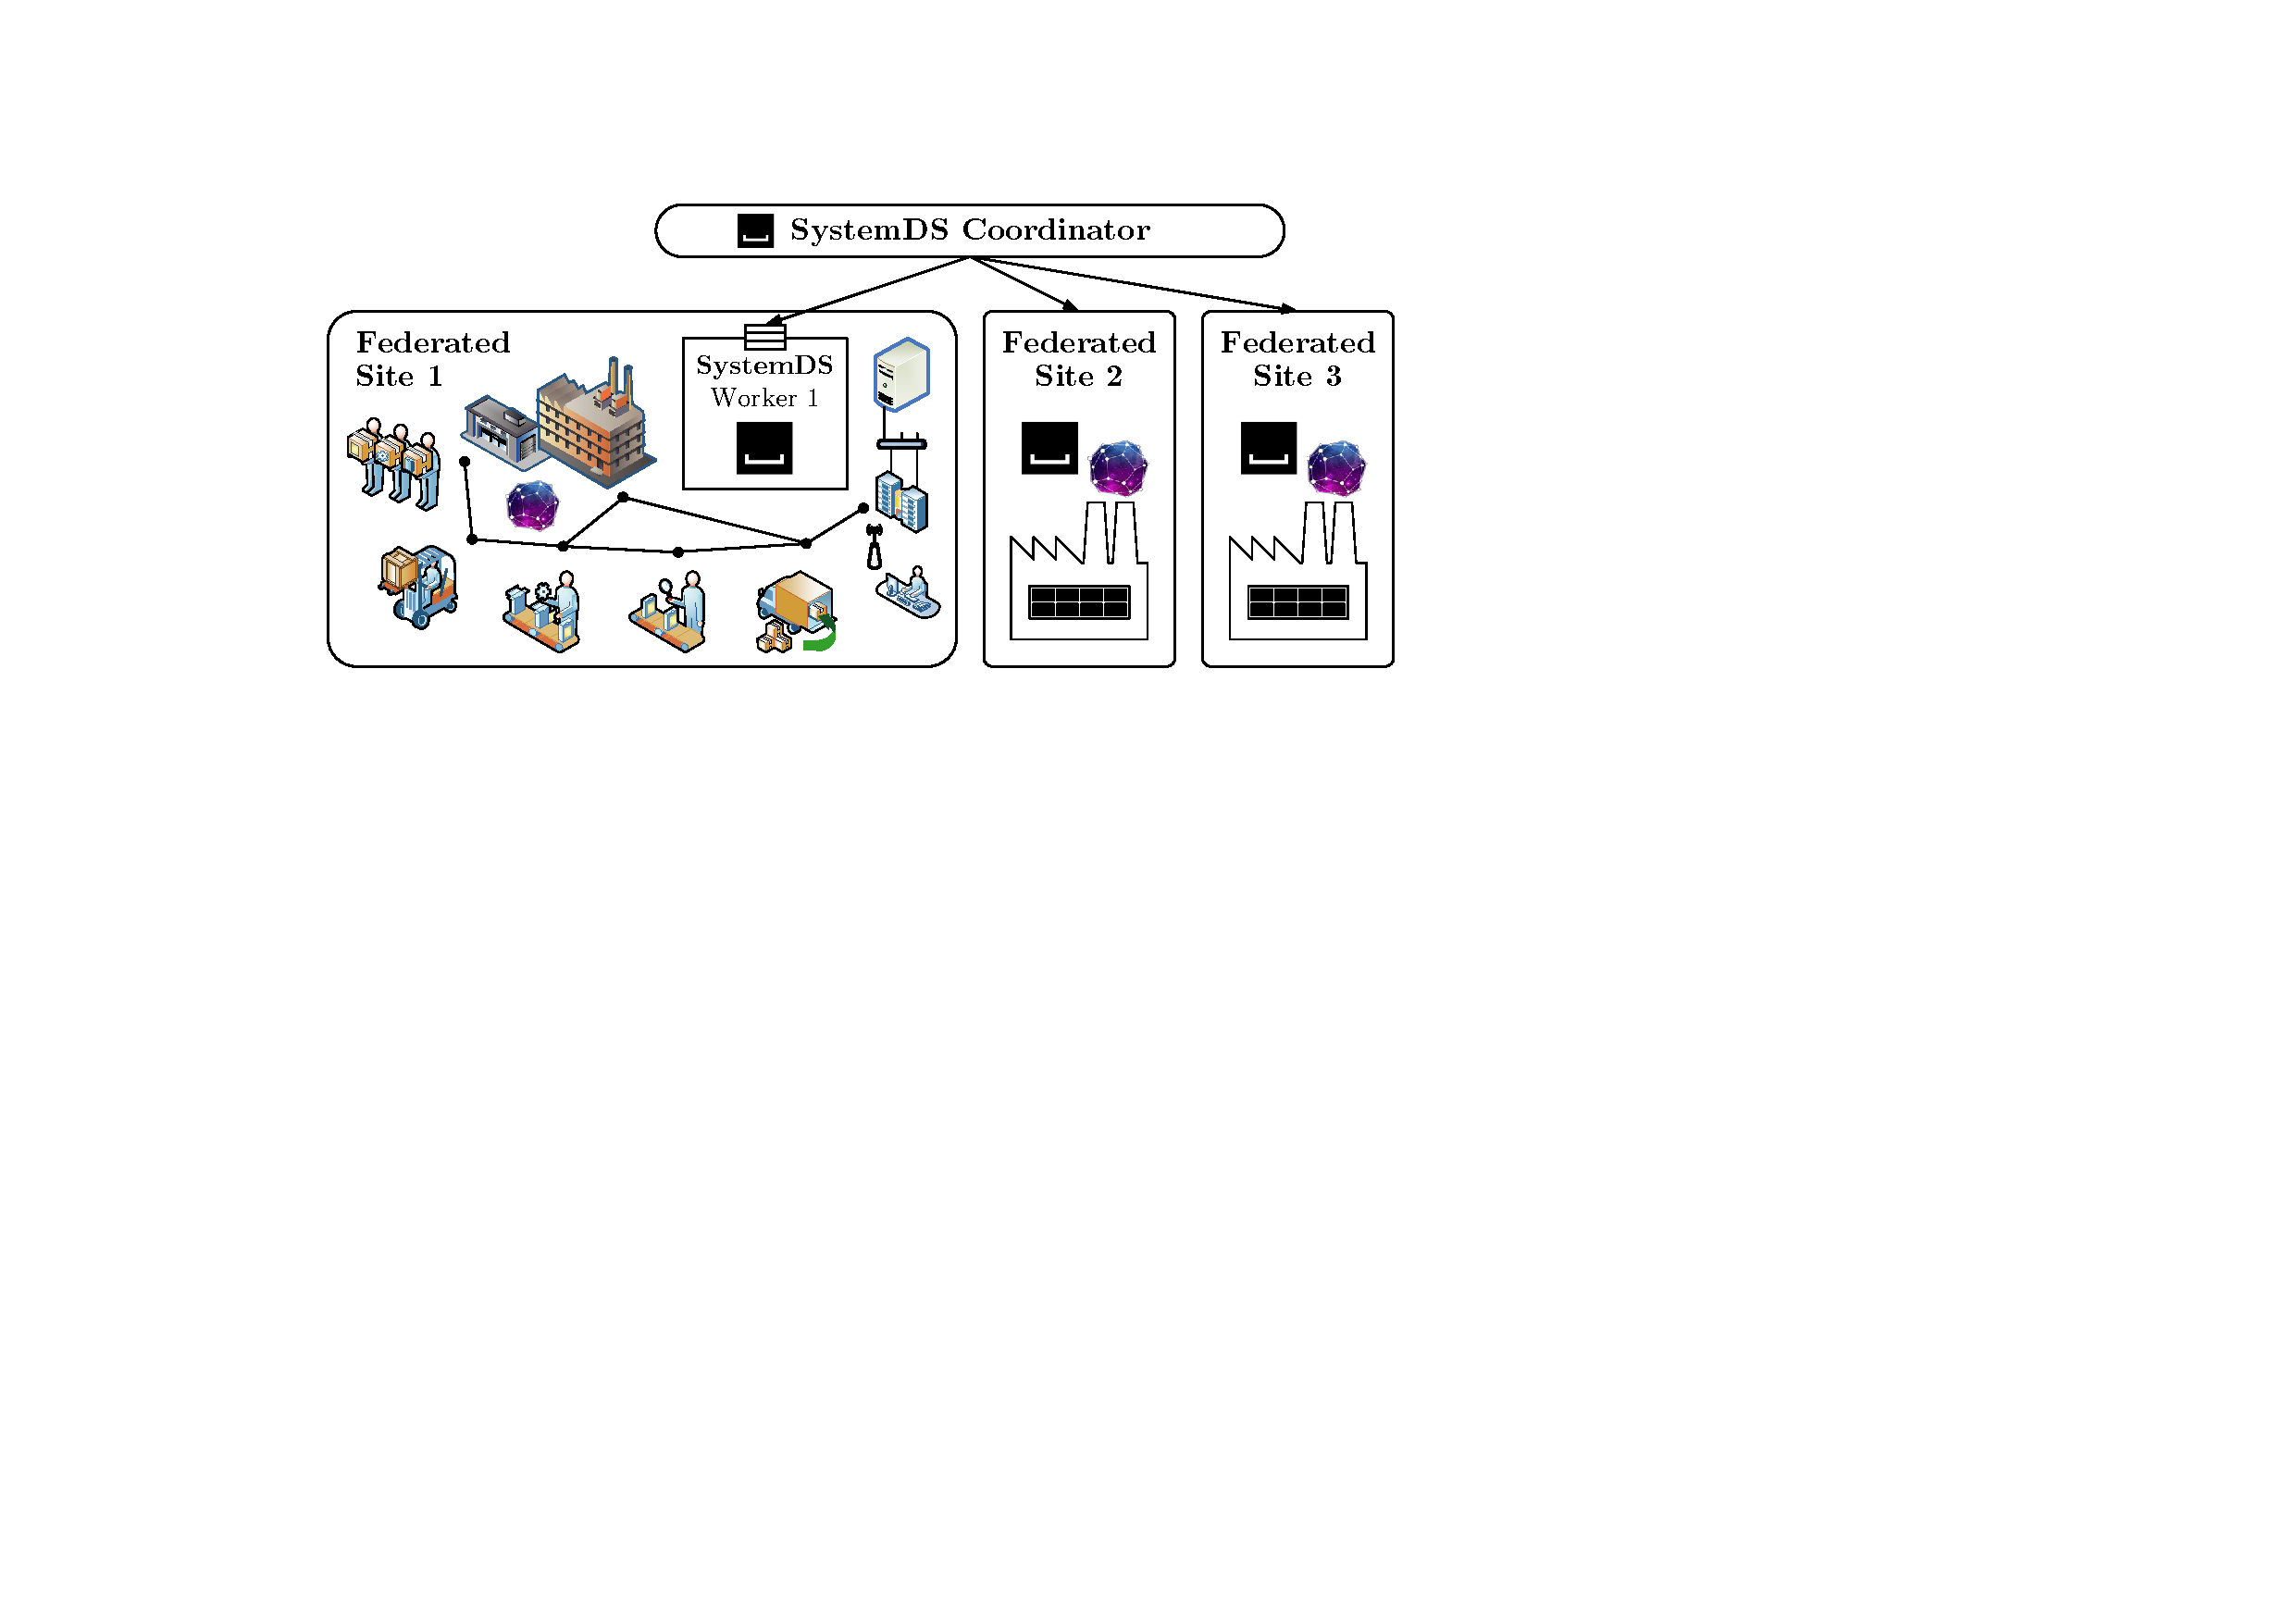
\includegraphics[width = 0.8\linewidth]{fig/fig04}
	\vspace{-0.25cm}
	\caption{\label{fig:preagg}Example Pre-aggregation in Compressed MatMult.}
	\Description{}
\end{figure}


% \begin{algorithm}
% 	\caption{LMM Algorithm}\label{alg:lmm}
% 	\Small
% 	\begin{algorithmic}
% 		\Require{$A$ , $G$} \Return{$R$}

% 		\State $(G^{m}, constRow) \gets Morph(G) $
% 		\State $P \gets allocatePreaggregate(|G^m|)$
% 		% \State $rowSums \gets rowSum(A) $
% 		\For{ $rb \gets 0$ to $nRow(A) / RowBlockSize$}
% 		\For{$cb \gets 0$ to $nCol(A) / ColBlockSize$}
% 		\For{$ i \gets 0$ to $|G^m|$}
% 		\State $P_i \gets G^m_i.preAggregate(A, rb, cb)$
% 		\EndFor
% 		\State $rowSums \gets rowSum(A, rb, cb)$
% 		\EndFor
% 		\State $R \gets R + G^m_i.mmDict(P_i)$
% 		\EndFor
% 		\State $R \gets R + rowSums.dot(constRow)$

% 		% \While{$Q.peek \neq NULL$ ,   $I^l \gets Q.poll$}
% 		% \State $I^r \gets Q.peek$ ,  $C \gets combine(I^l, I^r)$

% 		% \If{$cost(C)$ < $cost(I^l) + cost(I^r)$}
% 		% \State $Q.put(C)$
% 		% \Else
% 		% \State $P.add(I^l)$
% 		% \EndIf
% 		% \EndWhile
% 	\end{algorithmic}
% \end{algorithm}


\textbf{Left Matrix Multiplication:} We call the matrix multiplication $(\mat{A}\,\mathcal{G})$---where the left-hand-side input \mat{A} is uncompressed---a left matrix multiplication (LMM). Figure~\ref{fig:LeftMM} shows an LMM with two column groups.
For each column group, we compute the pre-aggregated $k \times d_i$ matrix $\mat{P}_i$ (via the already described vectorized pre-aggregation),
then matrix multiply $\mat{P}_i\,\mat{D}_i$, and finally, shift these results into the correct column positions of the output matrix $\mat{O}$.
Pre-aggregation for each column group is a linear scan of \mat{A}, but for large index structures $\mat{I}_i$, we can utilize cache-blocking
to reuse blocks of $\mat{I}_i$ from caches across multiple rows in \mat{A}. The more co-coding is applied, and/or the smaller the number of distinct items per group, the more we benefit from LMM pre-aggregation in terms of reduced floating point operations and data accesses. Multi-threaded LMM operations parallelize over column groups and rows in \mat{A} because they access disjoint output columns.

\begin{figure}[!t]
	\centering
	\subfigure[Left Matrix Multiply $(\mat{A}\,\mathcal{G})$.]{
		\label{fig:LeftMM}
\tikzset{indexstructure/.style={rectangle, draw, fill=black, minimum width=0.03cm, minimum height =1cm,
inner sep=0pt, text width =0mm}}
\tikzstyle{every node}=[font=\small]
\resizebox{0.3\textwidth}{!}
{
% \begin{tikzpicture}[node distance=0.35cm, transform shape]
\begin{tikzpicture}[node distance=0.35cm,font=\small]
    \node(left)[draw, thick, minimum width=2cm, minimum height=0.6cm]{Left Matrix};
    \node(preA1)[ pattern =crosshatch dots,  pattern color =black,right=of left, draw,  minimum width=1.1cm, minimum height=0.6cm,xshift=-0.1cm, yshift=0.1cm]{};
    \node(preA)[right=of left, draw, thick, fill=white, minimum width=0.8cm, minimum height=0.6cm]{$\mat{P}_i$};
    \node(out) [right=of preA, draw, thick, minimum width=1.cm, minimum height=0.6cm]{};
    
    \node(colG1)[fill=white, pattern =crosshatch dots,  pattern color =black,above=of out, draw, minimum width=0.38cm, minimum height=1.1cm,xshift=0.3cm]{};
    \node(colG) [above=of out, draw, thick, fill=white, minimum width=0.6cm, xshift=-0.2cm, minimum height=0.8cm]{$\mat{D}_i$};
    
    \node(colG1Out)[fill=white, pattern =crosshatch dots,  pattern color =black,right=of preA, draw, minimum width=0.38cm, minimum height=0.6cm,xshift=0.62cm]{};
    \node(colGOut)[right=of preA, draw, thick, fill=white, minimum width=0.6cm, minimum height=0.6cm]{$O_n$};
    
    \node(idx1)[above=of preA, indexstructure]{};
    \node(idx)[above=of preA, indexstructure, xshift=-0.1cm, yshift=0.1cm]{};
    
    \draw[->](left) to [out=90, in = 125] node[above, xshift=-0.2cm] {PreAggregate}(preA1);
    \draw[->](idx) to [out=-130, in = 125] (preA1);
    
    \node(labelIndexStructure)[] at (0.5,2.2){Index structures};
    \draw[->](labelIndexStructure) to [out=-30, in=90] (idx.north);
    \draw[->](labelIndexStructure) to [out=-10, in=90] (idx1.north);
    
    \node(labelDictionary)[] at(2.4, 2.4){Dictionaries};
    \draw[->](labelDictionary) to [out=-20, in=90] (colG1.north);
    \draw[->](labelDictionary) to [out=-80, in=130] (colG.north west);
    
    \draw[->](preA.north east) to[out=35,in=135](colGOut.north west);
    \draw[->](colG.south west) to[out=-135,in=135] node[above, xshift=-0.3cm]{MM}(colGOut.north west);
    
    \draw[->](preA1.north east) to[out=35,in=135](colG1Out.north west);
    \draw[->](colG1.south west) to[out=-135,in=135](colG1Out.north west);
    
    \node at(-1.3,0){$k$};
    \node at(0,-.55){$n$};
    \node at(1.95,-.55){$d_i$};
    \node at(2.9,1.7){$\card{\mathcal{G}_i}$};
\end{tikzpicture}
}}
	% \hfill
	\subfigure[Right Matrix Multiply $(\mathcal{G}\,\mat{B})$]{
		\label{fig:RightMM}
\tikzset{indexstructure/.style={rectangle, draw, fill=black, minimum width=0.03cm, minimum height =1cm,
inner sep=0pt, text width =0mm}}

\tikzstyle{every node}=[font=\small]

\resizebox{0.3\textwidth}{!}
{
\begin{tikzpicture}[node distance=0.35cm, transform shape]

    \node(overlappingOut)[draw, minimum height =1.3cm, minimum width=2cm, yshift=-0.1cm, xshift=0.3cm]{};
    \node(right)[draw, thick, fill=white,
        minimum width=1cm, minimum height=0.8cm, text width =0.9cm] at (-2,1.2){Right Matrix};

    \node(outG1)[ pattern =crosshatch dots,  pattern color =black, draw,
        minimum width = 1cm, minimum height=1.1cm,
        yshift=-0.08cm, xshift = 0.1cm]{};
    \node(outG)[draw, thick, fill=white,
        minimum width = 1cm, minimum height= 0.8cm]{$\mat{P}_i$};

    \node(colG1)[left=of outG, pattern =crosshatch dots, pattern color =black, draw,
        minimum width=0.38cm, minimum height=1.1cm, yshift=-0.08cm, xshift = -0.1cm]{};
    \node(colG) [left=of outG,draw, thick, fill=white,
        minimum width=0.6cm, minimum height=0.8cm]{$D_n$};

    \node(rightSlice1)[above=of outG,draw,  pattern =crosshatch dots, pattern color =black, draw,
        minimum width = 1cm, minimum height= 0.38cm,  xshift = 0.1cm,yshift=0.24cm]{};
    \draw[->](colG1.north east) to[out=35,in=135](outG1.north west);
    \draw[->](rightSlice1.south west) to[out=-135,in=135](outG1.north west);
    \node(rightSlice)[above=of outG, draw, thick, fill=white,
        minimum width = 1cm, minimum height= 0.2cm]{$Right_n$};

    \draw[->](right) to [out=0, in = 125] node[above, xshift=-0.2cm] {Slice}(rightSlice1.north west);
    \draw[->](right) to [out=0, in = 125] (rightSlice.north west);

    \node(labelOO)[text width=1.8cm] at(1.,-1.2){Overlapping Output};
    \draw[->](labelOO) to [out=180, in=-130] (overlappingOut);
    \node(labelDictionary)[] at(-1.8, -1.){Dictionaries};
    \draw[->](labelDictionary) to [out=60, in=-110] (colG1);
    \draw[->](labelDictionary) to [out=80, in=-140] (colG.south west);

    \draw[->](colG.north east) to[out=35,in=135](outG.north west);
    \draw[->](rightSlice.south west) to[out=-135,in=135] node[above, xshift=-0.35cm, yshift=-0.1cm]{MM}(outG.north west);

    \node(idx1)[right=of outG, indexstructure, xshift=.1cm, yshift=-0.2cm]{};
    \node(idx)[right=of outG, indexstructure, xshift=.2cm, yshift=-0.1cm]{};
    \node(labelIndexStructure)[text width= 1cm] at (2.0,0){Shallow Copy Indexes};
    \draw[->](labelIndexStructure) to [out=140, in=90] (idx.north);
    \draw[->](labelIndexStructure) to [out=130, in=90] (idx1.north);

    \node at(-1.8,0){$d_i$};
    \node at(0.9,1){$\card{\mathcal{G}_i}$};
    \node at(0,1.8){$k$};
\end{tikzpicture}
}
}
	% \hfill
	\subfigure[Transpose-Self MM$(\mathcal{G}^{\top}\,\mathcal{G})$]{
		\label{fig:tsmm}
\tikzstyle{every node}=[font=\small]
\resizebox{0.3\textwidth}{!}
{

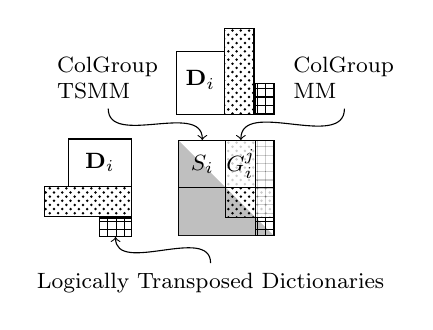
\begin{tikzpicture}[node distance=0.35cm, font=\footnotesize]

    \node(out) [ draw,  minimum width=1.21cm, minimum height=1.21cm]{};
    % gray diagonal.
    \draw[fill=gray, opacity=0.5] ([xshift=0.01cm, yshift=-0.01cm]out.north west)--([xshift=0.01cm, yshift=0.01cm]out.south west) -- ([xshift=-0.01cm, yshift=0.01cm]out.south east);



    % Above
    \begin{scope}[above=of out, xshift=-0.328cm,yshift=0.925cm]

        \node(colG2)[fill=white, pattern =grid, pattern color =black, draw, minimum width=0.2cm, minimum height=0.4cm,xshift=.82cm]{};
        \node(colG1)[fill=white, pattern =crosshatch dots,  pattern color =black, draw, minimum width=0.38cm, minimum height=1.1cm,xshift=0.49cm]{};
        \node(colG) [ draw,  fill=white, minimum width=0.6cm, minimum height=0.8cm]{};
        \node at ([yshift = -0.2cm]colG.center){$\mat{D}_i$};

    \end{scope}
    % left
    \begin{scope}[left=of out, xshift=-1.2cm, yshift=0.025cm]

        \node(colG2)[fill=white, pattern =grid, pattern color =black, draw, minimum width=0.4cm, minimum height=0.2cm,
            yshift=-0.52cm]{};
        \node(colG1)[fill=white, pattern =crosshatch dots,  pattern color =black, draw, minimum width=1.1cm, minimum height=0.38cm,
            yshift=-0.19cm]{};
        \node(colG) [ draw, fill=white, minimum width=0.8cm, minimum height=0.6cm,
            yshift=0.3cm]{$\mat{D}_i$};
    \end{scope}


    %top left
    \node(tsm)[ minimum width=0.6cm, minimum height=0.6cm, draw, anchor = north west] at(out.north west){$S_i$};

    %middle top
    \node[minimum height=0.6cm, minimum width=0.38cm,  pattern =crosshatch dots, draw,anchor = north west, pattern color =black, opacity=0.2]  at ([xshift=0.6cm]out.north west) {};
    \node(cgmme)[minimum height=0.6cm, minimum width=0.38cm, draw,anchor = north west,  label=center:$G_i^j$] at ([xshift=0.6cm]out.north west) {};


    % top right
    \node[minimum height=0.6cm, minimum width=0.2cm,  pattern =grid, pattern color =black, opacity=0.2, anchor= north west] at ([xshift=-0.02cm]cgmme.north east) {};
    \node[minimum height=0.6cm, minimum width=0.2cm,  draw, anchor= north west] at ([xshift=-0.02cm]cgmme.north east)  {};


    % middle right
    \node[minimum height=0.38cm, minimum width=0.2cm,  pattern =grid, pattern color =black, opacity=0.2,anchor= north west] at ([xshift=-0.02cm, yshift=0.02cm]cgmme.south east) {};
    \node[minimum height=0.38cm, minimum width=0.2cm,  pattern =crosshatch dots, pattern color =black, opacity=0.2,anchor= north west] at ([xshift=-0.02cm, yshift=0.02cm]cgmme.south east) {};

    % bottom right            
    \node[ minimum width=0.2cm, minimum height=0.2cm, draw, pattern =grid, pattern color =black, anchor = south east] at(out.south east){};

    % middle
    \node[ minimum width=0.38cm, minimum height=0.38cm, draw, pattern =crosshatch dots, pattern color =black, anchor = north west] at([xshift=-0.014cm, yshift=0.02cm]tsm.south east){};

    % ColGroup TSMM
    \node(cgt)[text width= 1.3cm]at(-1.5,1.4){ColGroup TSMM};
    \draw[->] (cgt) to [out=-90, in = 90](tsm);

    % ColGroup MM
    \node(cgmm)[text width = 1.3cm] at (1.5,1.4){ColGroup MM};
    \draw[->] (cgmm) to [out=-90, in = 90](cgmme);


    \node(mtdT)[] at(-0.2,-1.2){Logically Transposed Dictionaries};
    \draw[->](mtdT) to[out=90, in=-90] (colG2);

\end{tikzpicture}
}}
	\vspace{-0.35cm}
	\caption{\label{fig:ops}Types of Compressed Matrix Multiplication (with 2 and 3 column groups).}
	\Description{}
\end{figure}

\textbf{Morphing:} Some types of column groups are able to skip processing rows or columns for certain operations. We leverage such properties by changing the format---similar to the technique from MorphStore \cite{PattrickAJADW20}---of DDCFOR, SDC, SDCFOR, and SDCSingle groups before performing LMM. Using SDCFOR as an example, we simply take the reference tuple as a vector, subtract it from the dictionary, and return a SDCZero column group with the modified dictionary. We multiply \mat{A} and the column group using the preaggregate technique, and then add the vector scaled by row-sum of the left-hand-side matrix. In cases where multiple groups are morphed, their vectors are combined and processed together. This technique is also applied---with slight modifications---in decompression, right matrix multiply, and unary aggregates. This approach is virtually constructing an overlapping constant group for the entire matrix, transforming a single multiplication into a cheaper matrix multiplication, a row sum, and vector outer-product.

\textbf{Right Matrix Multiplication:} Similar to LMM, we call a matrix multiplication $(\mathcal{G}\,\mat{B})$---where the right-hand-side input \mat{B} is uncompressed---a right matrix multiplication (RMM). Figure~\ref{fig:RightMM} shows an example with two column groups. Our column-oriented compression and multiplication by \mat{B} from the right, provides an opportunity to preserve structural redundancy and thus, avoid unnecessary decompression (aggregation into an uncompressed output). The simple, yet very effective, key idea of our RMM is to only perform the vectorized pre-aggregation $\mat{P}_i = \mat{D}_i\,\mat{B}^{*}$ by multiplying the column group dictionaries with related rows in \mat{B}, and then store these pre-aggregates as new dictionaries of overlapping column groups. This way, we can leave the index structures $\mat{I}_i$ untouched and shallow-copy them into the compressed output representation, preserving the source redundancy. Each output column group now has dictionaries of size $d_i \times k$. The individual column groups compute, again independent (but now overlapping) outputs and thus, multi-threaded operations parallelize over column groups and columns of \mat{B}. In distributed environments with block-local matrix multiplications, the same RMM applies and the overlapping output can be preserved (if beneficial in size) even through serialization and shuffling.

\textbf{Transpose-Self Matrix Multiplication:} Transpose-self matrix multiplication (TSMM\footnote{TSMM is also known as BLAS syrk (symmetric rank-k update) or Gram matrix.}) $\mat{X}^{\top}\,\mat{X}$ or $\mat{X}\,\mat{X}^{\top}$---whose outputs is known to be symmetric---appears in many applications such as closed-form linear regression, co-variance and correlation matrices, PCA, and distance computations. CLA emulates TSMM again via slicing and repeated vector-matrix multiplications. In contrast, \name\ natively supports TSMM as shown in Figure~\ref{fig:tsmm}, as well as compressed-compressed matrix multiplications (with transposed left input), which are also commonly occurring in practice. A TSMM is composed of pairs of column group operations, where blocks on the diagonal are self-joins of column groups, while others are $\card{\mathcal{G}}\cdot(\card{\mathcal{G}}-1)/2$ combinations of column groups. First, a self-join of a column group computes (or reuses) the $d_i \times 1$ pre-aggregate $\mat{P}$ of tuple frequencies, and subsequently computes the results via an uncompressed TSMM $(\mat{D}\odot\mat{P})^{\top}\,(\mat{D}i)$, i.e., where rows of $\mat{D}$ are scaled by their frequencies. Second, for remaining blocks and compressed-compressed matrix multiplications, we adopt the strategy of LMM: pre-aggregation and matrix multiplication $\mat{P}_i\,\mat{D}_i$. However, given two compressed inputs, we can freely pick the pre-aggregation side and alternatively, do $(\mat{P}_j\,\mat{D}_j)^{\top}$. In any case, the pre-aggregate is computed without decompression and can exploit column-group characteristics (e.g., sparse, non-default, or constant encoding).

\textbf{Cost Analysis:} Apart from reduced I/O and memory-bandwidth requirements due to the smaller compressed size, compression can also reduce the number of floating point operations. In detail, Table~\ref{tab:cost} compares the asymptotic behavior of uncompressed matrix multiplications with related \name \ operations. Uncompressed LMM and RMM have both cubic complexity, where we ignore sparse linear algebra for the sake of simplicity. In contrast, compressed LMM and RMM have a complexity has depends on the data characteristics (distinct items and co-coding per column group). First, for LMM, we have two terms for pre-aggregation (only additions) and dictionary-based computation (additions and multiplications). With substantial co-coding (e.g., $\card{\mathcal{G}}=1 \wedge \card{\mathcal{G}_i}=m$) and few distinct items $d_i$, a much better complexity than cubic is possible ($\mathcal{O}(kn + km)$ instead of $\mathcal{O}(knm)$). In the worst-case, $\card{\mathcal{G}}=m$ and $d_i=n$, which gives $\mathcal{O}(knm)$ but with a higher constant factor. Second, RMM has only the second term of LMM and thus, we already benefit with less favorable data characteristics but the same worst-case guarantees apply, even with subsequent decompression. TSMM is more complex but the first term of the addition represents self-joins per column group (including pre-aggregation), and the second term enumerates pairs of column groups with two sub-terms for pre-aggregation and scaling. These cost functions, together with estimated or observed compression ratios, are also the basis for our workload-aware compression planning, allowing us to optimize for total execution time.

\begin{table}[!t]
  \centering \setlength\tabcolsep{12.5pt}
	\caption{\label{tab:cost}Complexity of Matrix Multiplications.}
	\vspace{-0.4cm}
	\begin{tabular}{ccc}
		\toprule
		     & \textbf{Uncompressed} & \textbf{\name}                                                                                               \\
		     & (dense)                               & (multiple, dense column groups)                                                                              \\
		\midrule
		LMM  & $\mathcal{O}\left(knm\right)$         & $\mathcal{O}\left(kn\card{\mathcal{G}} + k \sum_{i=1}^{\card{\mathcal{G}}}(d_i \card{\mathcal{G}_i})\right)$ \\
		RMM  & $\mathcal{O}\left(knm\right)$         & $\mathcal{O}\left(k \sum_{i=1}^{\card{\mathcal{G}}}(d_i \card{\mathcal{G}_i})\right)$                        \\
		TSMM & $\mathcal{O}\left(nm^2\right)$        & \hspace{-0.3cm}
		$\mathcal{O}\left(
			 {l} \sum_{i=1}^{\card{\mathcal{G}}}(n + d_i \card{\mathcal{G}_i}^2)+
					\sum_{i=1}^{\card{\mathcal{G}}}\sum_{j=i+1}^{\card{\mathcal{G}}}(n\card{\mathcal{G}_i} + \card{\mathcal{G}_i}d_j \card{\mathcal{G}_j})
				
			\right)$                                                                                                                                                \\
		\bottomrule
	\end{tabular}
\end{table}


% \textbf{Worst-case Complexity:}
% Recent theory work \cite{AbboudBBK20} presented impossibility results for efficient matrix-vector multiplications on grammar-compressed matrices such as Lempel-Ziv.
% In contrast, CLA's and \name's worst-case complexity is equal to the uncompressed case.
% First, given a compressed column C, the sparse encodings (SDC, OLE \&, RLE) require only $\text{distinct}(C)\leq \text{nrow}(C)$ multiplications, and $\text{nnz}(C)$ additions.
% The dense encoding DDC behaves similarly but requires scanning $\text{nrow}(C)$ instead of $\text{nnz}(C)$ code words.
% Second, if $\text{distinct}(C) < \text{nrow}(C)$, CLA reduces the number of multiplications, co-coding reduces the number of additions.
% Third, compression is only applied if the compressed size is smaller than uncompressed, which reduces memory bandwidth.

\subsection{Aggregations and Element-wise Operations}

Aggregations and element-wise operations are largely similar to CLA but with few extensions that leverage the design for redundancy exploitation and optimization for total execution time.

\textbf{Tuple Frequencies and Defaults:} Aggregations like $\text{sum}(\mat{X})$ or $\text{colSums}(\mat{X})$ pre-aggregate counts and then scale and accumulate the dictionary $\mat{D}_i$. In CLA, column group types like OLE only need to aggregate segment sizes, but DDC column groups still required a full scan of the index structures. In \name\, the most common column groups are DDC and SDC. By materializing the tuple frequencies, we can often reuse $\mat{P}_i$, yielding better asymptotic behavior. For matrix-scalar and matrix/row-vector operations---as used for standardization (e.g., $\mat{X}-\text{colMeans}(\mat{X})$---we further preserve the structural redundancy by handling default values in SDC column groups (e.g., replace zero by column mean), leaving the index structures unchanged.

\textbf{Handling Overlapped State:}
After right matrix multiplications, operations have to deal with---but can also leverage and propagate---overlapping state with partial sum semantics.
Generally, sum-product operations can be executed directly on overlapping state.
While left matrix multiplications directly apply, aggregations and element-wise operations require special treatment.
The list of extended operations includes full or column aggregations like sum or mean, but also matrix-scalar or matrix/row-vector multiplications and additions.
For matrix/row-vector addition and subtraction (e.g., $\mat{X}-\text{colMeans}(\mat{X})$, we can add a single overlapping column group (of constant columns),
whereas for $\mat{X}/\text{colSds}(\mat{X})$, we process all overlapping dictionaries via uncompressed matrix-vector operations.
Operations like min/max/pow or matrix-matrix operations are not supported in overlapping state because these types do not distribute over sums.

\textbf{Decompression:}
Unsupported \name\ operations or operations that cannot process overlapping state are then handled by decompression.
We use cache-conscious blocking for converting the column-compressed matrix into a row-major uncompressed matrix.
In contrast to update-fragment compaction during read in TileDB \cite{PapadopoulosDMM16} (latest writer wins),
we accrue the overlapping column group contributions into the output with $\mathcal{O}(nm\card{\mathcal{G}})$ time complexity (worst-case of $\card{\mathcal{G}}$ overlapping groups). Although decompression is expensive, it ensures robustness and allows controlling potential redundancy,
but if more efficient than full decompressions, we support partial decompressions to enable the operations to process sub-parts of the matrix at a time. 

\section{Workload-aware Compression}
\label{sec:workload}

\name\ aims to achieve broad applicability by redundancy exploitation and optimization for execution time.
Instead of compressing input matrices only according to data characteristics, we extract workload characteristics from the given LA program,
and compress candidate inputs and intermediates in a data- \emph{and} workload-aware manner (Section~\ref{sec:wlc1}),
and then leverage compressed data characteristics for a refined compilation of execution plans (Section~\ref{sec:wlc2}).

\subsection{Workload Trees and Compression}
\label{sec:wlc1}

Given a linear algebra program, workload-aware compression selects intermediates as compression candidates,
and for each candidate extracts a workload tree (a compact workload summary seen in Figure \ref{fig:wtree}),
evaluates its costs, and if valid for compression, injects a \texttt{compress} directive that utilizes the workload for fine-tuned (i.e., workload-aware) compression.

\textbf{Workload Trees:}
Many workloads in practice are complex LA programs with conditional control flow,
non-trivial function call graphs, and thousands of operations.
However, compressing an input or intermediate often affects only a small subset of data-dependent operations.
We introduce the notion of a \emph{workload tree} as a compact representation of these operations to simplify optimization.
A workload tree for a single candidate intermediate represents the program hierarchy of conditional control flow (branches and loops) as well as function calls as inner nodes,
and relevant compressed operations as leaf nodes.
Here, parent-child relationships represent containment.
For the sake of compactness, the tree comprises only inner nodes that contain at least one compressed operation.
Counting frequencies and costing is then an aggregation across hierarchy levels.
For loops, we multiply the costs by the number of iterations.
If the number of iterations is unknown (e.g., convergence-based loops),
we assume a constant 10 to reflect that operations inside the loop, are likely executed multiple times.
Some instructions are further multiplied by the dimensionality of the inputs, and if unknown during optimization, a multiplier of 16.

\begin{figure}[!t]
  \centering
  \includegraphics[width=0.8\linewidth]{fig/fig06}
  \vspace{-0.15cm}
  \caption{\label{fig:wtree}
  Example showing a user script that reads a feature matrix \mat{X} and label vector \mat{y},
  normalizes \mat{X} to mean 0 and standard deviation 1, and then trains an l2-regularized support vector machine.
  These functions are themselves linear-algebra scripts.
  Assuming \mat{X} as a compression candidate, we extract the workload tree at the right,
  which contains 2 function calls, 3 if branches,
  2 nested while loops and 8 compressed operations and 1 decompression.
  Aggregating the workload tree yields a cost summary for categories of operations.
  }
  % Workload Tree Extraction.
  \Description{}
\end{figure}

% \begin{example}[Example Workload Tree]
%   \label{ex:wtree} Figure~\ref{fig:wtree} shows an example user script that reads a feature matrix \mat{X} and label vector \mat{y},
%   normalizes \mat{X} to mean 0 and standard deviation 1, and then trains an l2-regularized support vector machine.
%   These functions are themselves linear-algebra scripts.
%   Assuming \mat{X} as a compression candidate, we extract the workload tree at the right,
%   which contains two function calls, three if branches,
%   two while loops and eight compressed operations and one decompression.
%   Aggregating this workload tree yields a cost summary (for categories of operations).
% \end{example}

\textbf{Workload Tree Extraction:}
Our initial candidate selection and optimization approach relies on heuristics.
We make a linear scan over the program, and extract compression candidates by operation type (e.g., persistent reads, comparisons, \texttt{ctable}, and rounding) as well as shape constraints (dimensions, and row/column ratios).
Together, these heuristics find good candidates while keeping the number of candidates low.
For each candidate, we then make a scan over the program and extract its workload tree by computing the transitive closure of derived compressed intermediates (based on operation types that are known to produce compressed outputs).
Again in a heuristic manner, we then evaluate individual candidates independently without considering joint effects of groups of compressed intermediates.
This extraction also descents into functions, but via stack-based identification includes only the first level of recursive function calls.
In this context, we prune the unnecessary extraction of workload trees for overlapping intermediates.
We perform this extraction at the end of inter-procedural analysis (IPA).
At this point, literals and size information have been propagated across the program and into amenable functions, and many simplifications have been performed.
In Figure~\ref{fig:wtree}, we would have propagated the shift, scale, and intercept flags, removed unnecessary branches, and inlined the scale function into the main program.

\textbf{Cost Evaluation:}
The cost summaries computed from the workload tree serve two purposes: for comparing uncompressed operations,
and for guiding compression planning.
We compute both frequencies and costs, where the latter utilizes the cost functions from Table~\ref{tab:cost}.
% The frequencies ignore size differences, but because many intermediates reflect the candidate shape---while row or column aggregations decompress---they represent the workload mix reasonably well.
We organize the cost summaries by categories of operations with different behavior in compressed space: (0) Decompression, (1) Overlapping Decompression, (2) LMM, (3) RMM, (4) TSMM, (5) Dictionary-Ops, and (6) Indexing-Ops.
Decompression is the frequency of regular decompressions,
while overlapping decompression converts the overlapping output into uncompressed form if operations
are not applicable on partial aggregates; both counts are multiplied by number of columns in each occurrence.
LMM is multiplied by the number of rows on the left, RMM multiplied by the number of columns on the right, and TSMM includes counts of compressed multiplications and transpose-self multiplications and is multiplied by the number of columns.
Dictionary operations can be performed directly on the compressed dictionaries (e.g., sum or element-wise scalar operations).
Finally, Indexing refers to slicing of batches or blocking during broadcasting.
If the cost evaluation suggests that compressing an intermediate may be beneficial, we make the cost summary globally available, and inject the related \texttt{compress} directive.
% \textbf{Compress/Decompress Directives:}
%  and place additional \texttt{decompress} directives if needed to handle cases that are difficult to decide at runtime.
% For example, Figure~\ref{fig:wtree} shows an RMM yielding a compressed intermediate \texttt{Xd} in overlapping state.
% This intermediate is used in the inner loop by an element-wise scalar multiplication but subsequently decompressed into non-overlapping state.
% In order to avoid decompression per iteration, we can place a \texttt{decompress} before the inner loop.

\textbf{Compression Planning:}
The \texttt{compress} directives injected into the execution plan, perform compression as described in Section~\ref{sec:compressalg}, but for workload-awareness get a cost summary. The workload mix influence the selection of column group types, co-coding decisions, and tuning for compression ratios.
During classification and co-coding, we estimate the column costs from the sample, and then use these costs to decide on column groupings instead of grouping purely for compression ratios.
However, including I/O costs also enables adapting the compression plans for large out-of-core datasets where good compression ratios are important to fit data in memory and/or reduce I/O. Local compression directly leverages the cost summaries, while for distributed compression, we serialize the cost summaries and compress blocks independently.

\textbf{Adaptive Compression:} In our federated learning backend \cite{Baunsgaard0CDGG21,Baunsgaard0IKLO22}, 
standing worker processes execute continuously incoming
operation requests from multiple tenants. \name\ also supports these
dynamically changing workloads by summarizing cost vectors of previously
executed operations and triggering asynchronous compression to adapt the
compressed representation when needed.


\subsection{Workload-aware Execution Planning}
\label{sec:wlc2}

In the context of hybrid runtime plans---composed of local in-memory, and distributed Spark operations---after compression, opportunities for compiling more efficient plans arise.
Specifically, we can compile operations on compressed intermediates to local operations, where uncompressed operations would exceed the memory budget and fallback to distributed runtime plans.

\textbf{Program Restructuring:} The challenge is that compression happens at runtime, and thus, the estimated and actual compressed size is unknown during initial compilation. Accordingly, we create---similar to data-dependent operators with unknown output shapes \cite{BoehmBERRSTT14}---artificial recompilation opportunities by splitting basic blocks after injected \texttt{compress} directives. If a block contains multiple, independent \texttt{compress} operators, we create a single cut for all.

\textbf{Compression-aware Recompilation:}
If an operator is marked for distributed operations due to unknown input/output dimensions or sparsity during initial compilation,
the entire DAG (basic block) is marked for recompilation during runtime.
Workload-aware compression leverages this infrastructure for obtaining the actual size of compressed in-memory matrices,
and propagating the compressed size bottom-up through the DAG.
With this updated size information, we can compile and execute refined partial execution plans.
Affected decisions include selected execution types (local vs Spark), and physical operators including broadcasting.



\newcolumntype{P}[1]{>{\centering\arraybackslash}p{#1}}

\section{Experiments}
\label{sec:Experiments}

Our experiments study \name\ in Apache SystemDS\footnote{All code and experiments are available open source in Apache SystemDS (\url{https://github.com/apache/systemds}) and our reproducibility repository (\url{https://github.com/damslab/reproducibility}).} in comparison with uncompressed operations (ULA), compressed linear algebra (CLA)~\cite{ElgoharyBHRR16, ElgoharyBHRR18} in Apache SystemML, and different data types in TensorFlow. We evaluate a variety of micro benchmarks, end-to-end ML algorithms, and hyper-parameter tuning; with local, distributed, and hybrid runtime plans.

\subsection{Experimental Setting}
\label{sec:setup}

\textbf{Hardware Setup:}
Our local and distributed experiments use a scale-out cluster of $1+6$ ($1+11$) nodes,
each having a single AMD EPYC 7443P CPU at $2.85$\,GHz (24 physical/48 virtual cores),
$256\gb$ DDR4 RAM at 3.2\,GHz, $1\times 480\gb$ SATA SSD,
$8\times 2\tb$ SATA HDDs (data) and Mellanox ConnectX-6 HDR/200\,Gb Infiniband. 
We use Ubuntu 20.04.1, OpenJDK Java 11.0.13 with JVM arguments \texttt{-Xmx110g -Xms110g -Xmn11g}, 
Apache Hadoop 3.3.4, and Apache Spark 3.2.0. The CLA baseline uses SystemML 1.2 with Spark 2.4 and equivalent configurations.
Some experiments marked with * were run on another cluster (for comparison) of $1+6$ nodes with AMD EPYC 7302 CPU at $3.0-3.3$~GHz (16/32 cores).
$128\gb$ DDR4 RAM at 2.933\,GHz, $2\times 480\gb$ SATA SSDs (system/home), $12\times 2\tb$ HDDs (data), and $2\times 10\text{Gb}$ Ethernet.

\textbf{Datasets:}
Since compression is strongly data-dependent, we exclusively use the real datasets shown in Table~\ref{tab:data}. This selection includes dense, sparse, and ultra-sparse datasets with common data characteristics.
All reported sizes and compression ratios refer to the size in memory using a sparsity threshold of 0.4 for uncompressed matrices.
US\,Census \cite{uci} is further used in an encoded form with binning/one-hot encoding for numerical, and recoding/one-hot encoding for categorical features, resulting in an increase from 68 to 378 columns, and the increased sparsity from $0.43$ to $0.18$, but with negligible change of the size in memory.
For large-scale experiments, we use a replicated versions of US\,Census\,Enc (up to 128x) which is roughly $290\gb$ and after densifying operations more than $950\gb$.
The Spark default configuration uses a storage fraction of 0.5, which gives an aggregate cluster memory of $6 \cdot 105\gb \cdot 0.5 = 315\gb$.
That way, we scale to data sizes that require I/O per iteration in uncompressed representation.

\begin{table}[!t]
	\centering \setlength\tabcolsep{15.2pt}
	\caption{\label{tab:data}Datasets {\normalfont($n$ Rows, $m$ Columns, $sp$ Sparsity)}.}
	\vspace{-0.4cm}
	\begin{tabular}{rrrrr}
		\toprule
		\multicolumn{1}{c}{\textbf{Dataset}} & $n$ ($\text{nrow}(\mat{X})$) & $m$ ($\text{ncol}(\mat{X})$) & \multicolumn{1}{c}{$sp$} & \multicolumn{1}{c}{Size} \\
		\midrule
		Airline78 \cite{airline}             & \num{14462943}               & 29                           & 0.54                     & $3.4\gb$                 \\ %3355402928
		Amazon \cite{amazon,HeM16}           & \num{8026324}                & \num{2330066}                & 1.2e-6                   & $1.22\gb$                \\ %1220001352
		Covtype \cite{uci}                   & \num{581012}                 & 54                           & 0.22                     & $127\mb$                 \\ %128635964
		Mnist1m \cite{infimnist}             & \num{1000000}                & 784                          & 0.25                     & $2.46\gb$                \\ %2461000104
		US\,Census \cite{uci}                & \num{2458285}                & 68 (378)                     & 0.43 (0.18)              & $1.34\gb$                \\ %1337307192
		US\,Census 128x                      & \num{314660480}              & 68 (378)                     & 0.43 (0.18)              & $289.5\gb$               \\ % 2261750120 * 128 = 289504015360
		\bottomrule
	\end{tabular}
\end{table}

\subsection{Compression Performance}

We first investigate the compression process itself in terms of compression times, compression ratios, and the influence of workload characteristics.

\begin{table} [!t] \setlength\tabcolsep{11.7pt}
  \vspace{-0.4cm}
	\caption{\label{tab:compressionTimes} Local Compression Times [Seconds] and Ratios.}
	\vspace{-0.4cm}
	\begin{tabular}{r|rr|rr|rr}
    \toprule
    \textbf{Dataset} & \multicolumn{2} {c|}{\textbf{CLA}}                            & \multicolumn{2}{c|}{\textbf{\name-Mem}} & \multicolumn{2}{c}{\textbf{\name}}                                                                                        \\
                     & \multicolumn{1} {c}{time}                                     & \multicolumn{1} {c|}{ratio}             & \multicolumn{1} {c}{time}          & \multicolumn{1} {c|}{ratio} & \multicolumn{1} {c}{time} & \multicolumn{1} {c}{ratio} \\
    \midrule
    Airline78        & \numprint{9.34} sec                                           & \numprint{10.22}                        & \numprint{1.74} sec                & \numprint{8.61}             & \numprint{2.08} sec       & \numprint{7.94}            \\
    Amazon           & \multicolumn{2} {c|}{\numprint{ 37.6} \textit{hours Crash}  } & \numprint{8.54} sec                     & \numprint{1.73}                    & \numprint{  3.77} sec       & \textit{Abort}                                         \\
    Covtype          & \numprint{1.10} sec                                           & \numprint{13.79}                        & \numprint{0.84} sec                & \numprint{14.24}            & \numprint{1.23} sec       & \numprint{13.99}           \\
    Mnist1m          & \numprint{7.25} sec                                           & \numprint{7.14}                         & \numprint{4.57} sec                & \numprint{6.09}             & \numprint{17.50} sec      & \numprint{4.41}            \\
    US Census        & \numprint{5.15} sec                                           & \numprint{35.38}                        & \numprint{1.16} sec                & \numprint{29.60}            & \numprint{1.15} sec       & \numprint{27.35}           \\
    US Census Enc    & \numprint{27.48} sec                                          & \numprint{41.03}                        & \numprint{5.78} sec                & \numprint{38.46}            & \numprint{6.54} sec       & \numprint{29.46}           \\
    \bottomrule
\end{tabular}


\end{table}

\textbf{Compression Ratios:} Starting with local single-node matrix compression, we compare \name~ optimized for memory (\name-Mem) and for workload (\name) with the existing CLA framework \cite{ElgoharyBHRR16,ElgoharyBHRR18}. The used workload is a fixed cost summary of left matrix multiplications that leads to extensive co-coding of columns. Table~\ref{tab:compressionTimes} shows the compression times and ratios for all datasets, where the ratios are calculated from the sizes of in-memory representations.
We attribute the minor differences to published CLA compression ratios \cite{ElgoharyBHRR18} (Airline78 7.44, Covtype 18.19, US\,Census 35.69) to different data preparation and sparse memory estimates.
Compared to CLA, \name yields worse compression ratios except for CovType, where \name's co-coding finds other column groups and uses new encoding types.
The lower compression ratios are due to the tuning for operations performance rather than size, and in practice, moderate absolute differences of large compression ratios have only little impact on size.
For example, compressing a $1\gb$ input with ratio 7 versus 6 yields only a difference of ~$24\mb$.
The Amazon dataset is an interesting case, where CLA runs out of memory due to group memoization during co-coding ($>2.7\cdot10^{12}$ pairs of columns). In contrast, \name~ aborts the compression early because the estimated total costs exceed the costs of ULA. Optimizing for memory in \name~ yields a low compression ratio for Amazon because of object overheads per column group, which do not exist in ULA's CSR representation.

\textbf{Compression Times:}
Table~\ref{tab:compressionTimes} further shows the compression times for all datasets.
% \name~ generally reduces compression times when optimizing for size (up to ~8x) and cost (up to ~3.7x), which make compression easier to amortize.
% The speed difference in \name-Mem US\,Census\,Enc is due to a reduction of the Grouping phase from 27 to 2.7 seconds.
\name~ generally reduces compression times when optimizing for size (up to ~4.7x) and cost (up to ~4.2x), which makes compression easier to amortize.
The speed difference in \name-Mem US\,Census\,Enc is due to a reduction of the grouping phase from 19 to 2.4 seconds.
When using workload-aware compression with a fixed cost summary that causes more grouping and compression,
only MNIST and US\,Census have significantly slower compression compared to optimizing for memory.
MNIST is slow because combining column groups have a large number of distinct values (each column contains up to 256 distinct values, and three columns together has up to $256^3$ distinct tuples).

\begin{table} [!t] \setlength\tabcolsep{10pt}
	\caption{\label{tab:sparkComp}Spark RDD Compression {\normalfont(Data: US\,Census\,Enc)}.}
	\vspace{-0.4cm}

	\begin{tabular}{r|cr|cr|c}
\toprule
          & \multicolumn{2} {c|}{\textbf{\name-Mem}} & \multicolumn{2} {c|}{\textbf{\name}} &                          \\
Blocksize & Ratio                                    & Total Size                           & Ratio & Total Size & ULA \\
\midrule
1K   	 &	\numprint{8.94} &	\numprint{225.58} MB &	\numprint{7.83} &	\numprint{257.36} MB &	\numprint{2.02} GB    \\
2K   	 &	\numprint{15.1} &	\numprint{143.49} MB &	\numprint{10.9} &	\numprint{198.55} MB &	\numprint{2.17} GB    \\
16K   	 &	\numprint{26.6} &	\numprint{81.68} MB &	\numprint{23.3} &	\numprint{93.36} MB &	\numprint{2.17} GB    \\
64K   	 &	\numprint{29.9} &	\numprint{72.74} MB &	\numprint{23.4} &	\numprint{92.96} MB &	\numprint{2.17} GB    \\
256K   	 &	\numprint{30.5} &	\numprint{71.22} MB &	\numprint{24.5} &	\numprint{88.70} MB &	\numprint{2.17} GB    \\
\bottomrule
\end{tabular}

\end{table}

\textbf{Compression Ratio Spark:}
For distributed operations, matrices are represented as Spark resilient distributed datasets (RDD) \cite{ZahariaCDDMMFSS12}---i.e.,
distributed collections of key-value pairs---with values being fixed-size matrix blocks of size $b \times b$ (except boundary blocks).
These blocks are compressed independently with separate compression plans and dictionaries.
The default block size is $b=1\text{K}$ ($8\mb$ dense blocks), but sparsity and compression warrant larger blocks.
Table~\ref{tab:sparkComp} varies this block size $b$ for US\,Census, and reports the size of \name-Mem, \name, and uncompressed (ULA) RDDs (from Spark's cached RDD-infos).
With small blocks, there is larger variability of compression, and increasing block sizes give better ratios while also stabilizing the resulting compression plans.
Overall, \name~ yields good compression ratios even with small $b$ and approaches local compression ratios with larger $b$.
For the remaining experiments, we use a block size of $b=16\text{K}$.


\subsection{Operations Performance}
\label{sec:OperationPerformance}

In a second series of micro-benchmarks, we compare the runtime of \name~ with ULA and CLA operations.
While CLA was designed for operations performance close to uncompressed and benefits from keeping large datasets in memory,
\name~ aims to improve performance more generally, even for in-memory settings and keep performance stable even if the input data is densified.
% Here, we focus on common aggregations, element-wise matrix-vector operations, small sequences of operations, as well as left, right, and transpose-self matrix multiplications.
We compare using both original and densified by simply adding 1 to all cells.

\textbf{Aggregations:} Figure~\ref{exp:sum} shows the results for computing the aggregate $\text{sum}(\mat{X})$. CLA processes each column group in parallel, aggregates individual sums, and combines them into the result. ULA uses multi-threading with sequential scans of row partitions.
By memorizing the frequencies of tuples, \name~ executes purely on the column group dictionaries without scanning their indexes because of memoization.
Without memoization, the execution time increase according to the complexity of scanning the index structures.
For instance, we observed no penalty in case of Census\,enc, while 60x performance drop in Census for \name.
When densifying, in Figure~\ref{exp:sumDense}, CLA and \name~ retain their performance while ULA's performance worsen.
For column aggregations (Figure~\ref{exp:colSum} and \ref{exp:colSumDense}), CLA is slower than ULA because CLA's DDC colSums is not specialized for DDC1 and DDC2 and thus, performs a lookup of dictionary values for each encoded cell.

\begin{figure}[!t]
	\centering
	\subfigure[Sum Original]{\label{exp:sum}\includegraphics[width= 0.47 \linewidth]{\source/microbenchmark/ua/sum_dams-so001.pdf}}\hfill
	\subfigure[Sum Dense]{\label{exp:sumDense}\includegraphics[width= 0.47 \linewidth]{\source/microbenchmark/ua/sum+_dams-so001.pdf}}\hfill~\vspace{-0.3cm}\\
	\subfigure[ColSums Original]{\label{exp:colSum}\includegraphics[width= 0.47 \linewidth]{\source/microbenchmark/ua/colsum_dams-so001.pdf}}\hfill
	\subfigure[ColSums Dense]{\label{exp:colSumDense}\includegraphics[width= 0.47 \linewidth]{\source/microbenchmark/ua/colsum+_dams-so001.pdf}}~\vspace{-0.4cm}\\
	% \subfigure[Plus Original]{\label{exp:plus}\includegraphics[width= 0.49 \linewidth]{\source/microbenchmark/sc/plus_dams-so001.pdf}}\hfill
	% \subfigure[Div Row-vector Dense]{\label{exp:divVectorDense}\includegraphics[width= 0.49 \linewidth]{\source/microbenchmark/ua/divvector+_dams-so001.pdf}}~\vspace{-0.3cm}\\
	\caption{\label{exp:opsua}Operations Performance Aggregate.}
	\Description{ microbenchmarks }
  \vspace{-0.4cm}
\end{figure}

\begin{figure}[!t]
	\subfigure[Plus Scalar, Original]{\label{exp:plus}\includegraphics[width= 0.47 \linewidth]{\source/microbenchmark/sc/plus_dams-so001.pdf}}\hfill
	\subfigure[Div Row-vector, Dense]{\label{exp:divVectorDense}\includegraphics[width= 0.47 \linewidth]{\source/microbenchmark/ua/divvector+_dams-so001.pdf}}~\vspace{-0.4cm}\\
	\caption{\label{exp:opsscalar}Operations Performance Scalar.}
	\Description{ microbenchmarks }
\vspace{-0.4cm}
\end{figure}


% \textbf{Element-wise Operations:} Figure~\ref{exp:plus} shows the performance of adding a scalar value to each matrix cell. We observe extreme speedups of up to 4984x because \name\ avoids modifying dictionaries where possible. Figures~\ref{exp:divVectorDense} shows similar improvements for matrix-vector (column vector) element-wise operations. Specifically, we analyze $\mat{X}/\mat{v}$ on sparse and dense representations, where we chose division because it forces modifications of the dictionaries. We still see speedups of about three orders of magnitude (1766x).
\textbf{Element-wise Operations:} Figure~\ref{exp:plus} shows the performance of adding a scalar value to each matrix cell. We observe extreme speedups of up to \numprint{10766}x because \name\ avoids modifying dictionaries where possible. Figures~\ref{exp:divVectorDense} shows similar improvements for matrix-vector (row vector) element-wise operations. Specifically, we analyze $\mat{X}/\mat{v}$ on sparse (not shown) and dense representations, where we chose division because it forces modifications of the dictionaries. We still see speedups of about three orders of magnitude (\numprint{2047}x).

\textbf{Left Matrix Multiplication (LMM):}
Left, right, and transpose-self matrix multiplications are key operations in many ML algorithms.
In the following, we first evaluate these operations independently.
Figure~\ref{exp:LMM} shows the results of left matrix multiplications for all datasets, where the uncompressed left-hand-side has 16 rows.
CLA emulates this matrix-matrix multiplication via 16 vector-matrix multiplications.
We observe \name~ performance comparable to multi-threaded ULA (sparse and dense) with improvements
for Covtype, US\,Census, and US\,Census\,Enc,
but a moderate slowdown for Airlines and a significant slowdown for MNIST.
LMM also shows a major performance difference when optimizing for memory versus optimizing for operations, which is especially noticeable in US\,Census\,Enc.
In contrast, for datasets with smaller potential for co-coding like Airline, there is no difference.
Figure~\ref{exp:mmlscale} shows results on US\,Census\,Enc with varying number of rows in the left-hand-side.
CLA performs similar to \name~ at a single row, but when rows increase CLA's performance decrease to the same as ULA due to the lack of native matrix-matrix support.
CLA is worse at utilizing more threads, while \name~ and ULA scale better.
For ULA and \name-Mem, there is a change in parallelization strategies after 16 rows.
In contrast, \name~ yields between half and one order of magnitude speedups for all \#rows configurations.

\begin{figure}[!t]
	\subfigure[16 row LMM]{\label{exp:LMM}\includegraphics[width= 0.47  \linewidth]{\source/microbenchmark/mm/16_mml_dams-so001.pdf}}\hfill
	\subfigure[LMM Census Enc Scaling]{\label{exp:mmlscale}\includegraphics[width= 0.47  \linewidth]{\source/microbenchmark/mm/mml_census_dams-so001.pdf}}~\vspace{-0.4cm}\\

	\caption{\label{exp:opsLMM}Operations Performance Left Matrix Multiplication.}
	\Description{ microbenchmarks }
\end{figure}

\begin{figure}[!t]
	\subfigure[16 col RMM]{\label{exp:RMM}\includegraphics[width= 0.47  \linewidth]{\source/microbenchmark/mm/16_mmr_dams-so001.pdf}}\hfill
	\subfigure[RMM Census Enc Scaling]{\label{exp:mmrscale}\includegraphics[width= 0.47  \linewidth]{\source/microbenchmark/mm/mmr_census_dams-so001.pdf}}~\vspace{-0.4cm}\\
	\caption{\label{exp:opsRMM}Operations Performance Right Matrix Multiplication.}
	\Description{ microbenchmarks }
	\vspace{-0.4cm}
\end{figure}

\textbf{Right Matrix Multiplication (RMM):}
In contrast to LMM, the right matrix multiplication creates outputs of overlapping column groups with a shallow copy of the index structures.
Figure~\ref{exp:RMM} shows the results for all datasets, where we observe \name~ speedups between
% 34x to 656x
53x to \numprint{1528}x
because of the deferred aggregation across column groups.
Figure~\ref{exp:mmrscale} then shows the scaling with increasing number of columns in the uncompressed right-hand-side.
CLA shows equal performance to uncompressed in the single column case but scales worse then ULA, again due to the lack of native matrix-matrix multiplication.
\name's RMM exhibits better asymptotic behavior due to its dictionary-centric operations,
% yielding speedups >$15000$x for 512 columns.
yielding speedups >\numprint{13000}x for 512 columns.

\begin{figure}[!t]
	\subfigure[TSMM Sparse]{\label{exp:tsmm}\includegraphics[width= 0.47  \linewidth]{\source/microbenchmark/ua/tsmm_dams-so001.pdf}}\hfill
	\subfigure[TSMM Dense]{\label{exp:tsmmDense}\includegraphics[width= 0.47  \linewidth]{\source/microbenchmark/ua/tsmm+_dams-so001.pdf}}~\vspace{-0.4cm}\\
	\caption{\label{exp:opsTSMM}Operations Performance Transpose Self Matrix Multiplication.}
	\Description{ microbenchmarks }
	\vspace{-0.4cm}
\end{figure}

\textbf{Transpose-Self Matrix Multiplication (TSMM):} Figures~\ref{exp:tsmm} and \ref{exp:tsmmDense} show the results of TSMM operations as used for computing PCA, direct-solve linear regression, as well as covariance and correlation matrices.
We observe speedups on all datasets except MNIST, where \name\ yields a substantial slowdown, especially for sparse inputs.
The TSMM performance is largely dependent on the number of column groups, their number of distinct items, and thus,
co-coding decisions. MNIST has a high number of columns, with high cardinality, and low correlation between columns.

\begin{figure}[!t]
	\subfigure[Scale and Shift Sparse]{\label{exp:scaleShift}\includegraphics[width= 0.47  \linewidth]{\source/microbenchmark/ua/scaleshift_dams-so001.pdf}}\hfill
	\subfigure[Euclidean MinDist 16 Points Dense]{\label{exp:euclideanDense}\includegraphics[width= 0.47  \linewidth]{\source/microbenchmark/mm/16_euclidean+_dams-so001.pdf}}~\vspace{-0.4cm}\\
	\caption{\label{exp:opsseq}Operations Performance Sequence.}
	\Description{ microbenchmarks }
\end{figure}

\textbf{Operation Sequences:}
As final micro benchmark use cases, we evaluate two sequences of operations. First, \emph{scale and shift} in Figure~\ref{exp:scaleShift}
performs a shifting $\mat{Y} = \mat{X} - (\text{colSums}(\mat{X})/\text{nrow}(\mat{X}))$ and scaling $\mat{Z} = \mat{Y} / \sqrt{\text{colSums}(\mat{Y}^2)/(\text{nrow}(\mat{Y})-1)}$.
This sequence is a common normalization step (standard-scaler) of the input data but has the negative side effect of densifying the input data.
% \name~ improves performance up to  a best case of 11924x. Second, we compute the minimum Euclidean distances via $\mat{D} = -2 * (\mat{X} \times t(\mat{C})) + t(rowSums(\mat{C}^2))$, followed by $\mat{d} = rowMins(\mat{D})$ (which forces a decompression from overlapping state). Here, $\mat{D}$ are the Euclidean distances of each row in \mat{X} to the coordinates \mat{C}. This expressions is used, for instance, in K-Means clustering. \name~ shows performance up to 14.5x faster compared to ULA in all cases except MNIST.
\name~ improves performance up to a best case of \numprint{15399}x. Second, we compute the minimum Euclidean distances via $\mat{D} = -2 * (\mat{X} \times \text{t}(\mat{C})) + \text{t}(\text{rowSums}(\mat{C}^2))$, followed by $\mat{d} = \text{rowMins}(\mat{D})$ (which forces a decompression from overlapping state). Here, $\mat{D}$ are the Euclidean distances of each row in \mat{X} to the centroids \mat{C}. This expressions is used, for instance, in K-Means clustering. \name~ shows performance up to 11.3x faster compared to ULA in all cases except MNIST.

\begin{table} [!t] \setlength\tabcolsep{17.4pt}
	\caption{\label{tab:expOverlap}RMM Overlap Sequence (Data: US\,Census\,Enc).}
	\vspace{-0.4cm}
	\begin{tabular}{r|r|r|r|r}
    \toprule
                   & \textbf{I/O}        & \textbf{Comp}        & \textbf{RMM}          & \textbf{Total}        \\
    \midrule
    SystemML - ULA & \numprint{0.84} sec & ---                  & \numprint{188.40} sec & \numprint{190.03} sec \\
    SystemML - CLA & \numprint{0.88} sec & \numprint{24.34} sec & \numprint{374.13} sec & \numprint{401.27} sec \\
    SystemDS - ULA & \numprint{0.81} sec & ---                  & \numprint{189.27} sec & \numprint{190.42} sec \\
    \name-No OL    & \numprint{0.76} sec & \numprint{3.97} sec  & \numprint{189.59} sec & \numprint{195.51} sec \\
    \name-Mem      & \numprint{0.80} sec & \numprint{8.00} sec  & \numprint{0.38} sec   & \numprint{9.72} sec   \\
    \name          & \numprint{0.78} sec & \numprint{3.93} sec  & \numprint{0.42} sec   & \numprint{5.69} sec   \\
    \bottomrule
\end{tabular}


\end{table}

\textbf{Overlap:} Leveraging the overlapping output from RMM without compaction shows significant improvements in Figures \ref{exp:RMM} and \ref{exp:opsseq}.
However, overlapping representations are most beneficial in chains of RMMs. Table \ref{tab:expOverlap} shows the end-to-end runtime for a sequence of $10$ RMM of size $k=512$, representative for processing $10$ fully-connected layers of size $512$ with no activation.
CLA is slower than ULA in this scenario because it is falling back to vector matrix compressed operations for the first multiplication.
\name~ with no overlapping is slower because the first right multiplication decompress, but it does show close to ULA performance.
% of its compression overhead, non-native matrix-matrix multiplications, decompressed intermediates and ULA operations after the first RMM.
%and finally because the subsequent uncompressed MM are worse at utilizing the cores
%dropping average cores utilized from $15.6$ to $8.6$ --> likely due to allocations.
\name~ with overlapping column groups push the compressed index structures through the entire chain of RMMs, improving performance irregardless of optimizing for memory or workload, with a slight advantage to workload.


\begin{table} [!b] \setlength\tabcolsep{8pt}
	\caption{ \label{tab:workload} \name \ Workload TOPS (Data: US\,Census\,Enc).}
	\vspace{-0.4cm}
	\begin{tabular}{r|rr|rrrr}
    \toprule
                   & \multicolumn{2} {c|}{\textbf{ULA}} & \multicolumn{4} {c}{\textbf{\name}}                                                                                                                  \\
    Op ($100\times$) & \multicolumn{1}{c}{TOPS}           & \multicolumn{1}{c|}{Time}           & \multicolumn{1}{c}{Est. TOPS} & \multicolumn{1}{c}{TOPS} & \multicolumn{1}{c}{Comp} & \multicolumn{1}{c}{Time} \\
    \midrule
    SUM & 3.38e+10  & \numprint{2.25} sec & 1.29e+05  & 1.14e+05 & \numprint{4.60} sec  & \numprint{0.08} sec \\
    SUM Dense & 1.90e+11  & \numprint{8.96} sec & 1.31e+05  & 1.14e+05 & \numprint{4.65} sec  & \numprint{0.07} sec \\
    RMM-256 & 2.81e+13  & \numprint{156.97} sec & 2.13e+07  & 1.94e+07 & \numprint{4.74} sec  & \numprint{0.25} sec \\
    LMM-256 & 4.28e+12  & \numprint{185.69} sec & 6.87e+11  & 7.14e+11 & \numprint{7.22} sec  & \numprint{53.76} sec \\
    TSMM & 6.32e+12  & \numprint{111.12} sec & 9.83e+11  & 9.98e+11 & \numprint{7.19} sec  & \numprint{16.91} sec \\
    ScaleShift & 7.47e+11  & \numprint{3216.21} sec & 4.08e+05  & 3.42e+05 & \numprint{4.89} sec  & \numprint{0.36} sec \\
    Euclidean-256 & 4.80e+13  & \numprint{308.85} sec & 8.61e+11  & 9.04e+11 & \numprint{7.87} sec  & \numprint{78.55} sec \\
    \bottomrule
    \end{tabular}

\end{table}

\textbf{Computation Cost:} Table \ref{tab:workload} shows the \name~ workload analysis of different micro benchmarks on Census\_Enc.
This experiment shows the estimated Theoretical Operations (TOPS), calculated from the cost vectors and compression schemes.
We compare the estimated TOPS for uncompressed operations (on the left) with \name's estimated TOPS extracted from the sample and co-coding decisions, as well as the estimated TOPS after compression (on the right). We observe that the estimated TOPS from the sample is close to the actual TOPS, indicating good estimation accuracy and thus, meaningful costs. We also show the compression time (Comp) and the runtime (Time) for executing 100 repetitions of the given operation (Op $100\times$). There are some micro benchmarks that show disproportionate scaling of runtimes compared to TOPS. With small execution times, moderate discrepancies are expected because of various unaccounted overheads in both ULA and \name. For TSMM and LMM, the differences are due to output allocation, memory bandwidth limitations, and index structure lookups. Although the runtime discrepancies are sub-par, we found that our TOPS estimation provides a good balance of simplicity and reflecting key differences relevant for compression. More sophisticated cost estimators are, however, interesting future work.

% \subsection{Computation Cost}
% Figure~\ref{exp:censusBreakdown} shows how optimizing for cost or memory changes the compression. Each plot is split into two parts: left the individual columns and right the co-coded column groups. First, the left plot shows cost in Tera Operations (TOPS), because FLOPs is not a good measure here since many operations are index lookups and bit shifting. We compare estimated and actual TOPS, which do not represent real instructions but abstract cost units our cost model is based on. Similar cost units can also be extracted for the uncompressed input and operations. Second, the right plot compares the estimated and actual size in memory when optimizing for size (\name-Mem). In both cases, the total score of a compression plan is the area under the curve. We see that co-coding reduces the number of column groups more when optimizing for computation cost---because it reduces the number operations---whereas when optimizing for size, co-coding decisions depend more on column correlations to be beneficial.

\subsection{End-to-End Algorithm Performance}
\label{sec:end-to-end}

% After having discussed the compression and operations micro-benchmarks,
% we can now turn to evaluating \name~ with workload-ware compression on end-to-end ML algorithms.
We use the following six algorithms to evaluate \name~ with workload-ware compression on end-to-end ML training:
K-Means for clustering;
principal component analysis (PCA) for dimensionality reduction;
multinomial (multi-class) logistic regression (MLogReg);
LM via conjugate gradient (lmCG), and via a direct solve method (lmDS) for linear regression;
as well as
l2-regularized support vector machines (L2SVM) for classification.
In theory, \name~ gives equal results to ULA but because of rounding errors in sequences of
FP64 operations and different parallelization strategies---present both, in ULA and \name---algorithms naturally execute with slight variations.
Therefore, algorithm parameters are set to ensure an equal number of iterations and operations.
We use the US\,Census\,Enc dataset and scale up by replication.
The replication maintains the statistics of the data,
and is not an issue for distributed execution, where blocks are compressed independently.
The local influence is limited to constant dictionary sizes, and replication is not actively exploited by \name.


\begin{table}[!t]
	\setlength\tabcolsep{10pt}
	\centering
	\caption{\label{tab:end2end}Workload-awareness on Local End-to-End Algorithms (Data: US\,Census\,Enc)}
	\vspace{-0.4cm}

	\begin{tabular}{r|r|rr|rr}
    \toprule
                     & \textbf{ULA}        & \multicolumn{2}{c|}{\textbf{\name-Mem}} & \multicolumn{2}{c}{\textbf{\name}}                                             \\
                     & Time                & Comp                                    & Time                               & Comp                & Time                \\
    \midrule
    \textbf{K-Means} &	\numprint{51.6} sec &	\numprint{4.2} sec &	\numprint{46.2} sec &	\numprint{6.2} sec &	\numprint{27.1} sec  \\
    \textbf{PCA}     &	\numprint{12.7} sec &	\numprint{4.0} sec &	\numprint{10.4} sec &	\numprint{6.0} sec &	\numprint{9.0} sec  \\
    \textbf{MLogReg} &	\numprint{32.0} sec &	\numprint{4.5} sec &	\numprint{32.5} sec &	\numprint{7.2} sec &	\numprint{26.0} sec  \\
    \textbf{lmCG}    &	\numprint{19.8} sec &	\numprint{5.0} sec &	\numprint{20.7} sec &	\numprint{6.4} sec &	\numprint{18.6} sec  \\
    \textbf{lmDS}    &	\numprint{15.6} sec &	\numprint{5.7} sec &	\numprint{15.5} sec &	\numprint{6.1} sec &	\numprint{14.3} sec  \\
    \textbf{L2SVM}   &	\numprint{38.9} sec &	\numprint{6.5} sec &	\numprint{45.2} sec &	\numprint{6.2} sec &	\numprint{36.5} sec  \\
    \bottomrule
    \end{tabular}
    

\end{table}%

\begin{table}[!t]
	\centering
	\setlength\tabcolsep{10pt}
	% \captionsetup{width=0.4\textwidth}
	\caption{\label{tab:expCLAEndToEnd}L2SVM (without scale\&shift, 60 iterations, Data: US\,Census\,Enc)}
	\vspace{-0.4cm}

	
\begin{tabular}{r|r|r|r|r||r}
    \toprule
                   & \multicolumn{4}{c||}{Local {\tiny(1x)}} & Distributed {\tiny(256x)}                                                                                   \\
    \midrule
                   & \textbf{I/O}                            & \textbf{Comp}             & \textbf{L2SVM}      & \textbf{Total}      & \multicolumn{1}{c}{ \textbf{Total}} \\

    \midrule
    SystemML - ULA & \numprint{1.6} sec                      & ---                       & \numprint{36.7} sec & \numprint{38.4} sec & \numprint{5689.6} sec               \\
    SystemML - CLA & \numprint{1.5} sec                      & \numprint{32.8} sec       & \numprint{31.7} sec & \numprint{66.0} sec & \numprint{4722.7} sec               \\
    SystemDS - ULA & \numprint{1.6} sec                      & ---                       & \numprint{19.3} sec & \numprint{20.9} sec & \numprint{2849.1} sec               \\
    \name-Mem      & \numprint{1.4} sec                      & \numprint{6.0} sec        & \numprint{21.3} sec & \numprint{28.7} sec & \numprint{2300.4} sec               \\
    \name          & \numprint{1.6} sec                      & \numprint{7.9} sec        & \numprint{15.9} sec & \numprint{25.3} sec & \numprint{2294.9} sec               \\
    \bottomrule
\end{tabular}


\end{table}%

\textbf{Local Execution:}
Table~\ref{tab:end2end} shows the results algorithms fit in-memory.
\name~ yields moderate but consistent improvements, or at worst (e.g. L2SVM, lmDS) comparable performance.
% Observing improvements of 36\% for MLogReg, 48\% for K-Means (iterative algorithms), and 27\% for PCA (non-iterative algorithm) is remarkably because this includes online compression. Underlying reasons are fast compression that is easier to amortize and redundancy exploiting operations.
Observing improvements on all algorithms most notably 19\% for MLogReg, 47\% for K-Means (iterative algorithms), and 29\% for PCA (non-iterative algorithm) is remarkably because this includes online compression.
Underlying reasons are fast compression that is easier to amortize and redundancy exploiting operations.
The algorithms L2SVM, lmCG, and lmDS all perform very close to ULA.

\textbf{CLA Comparison:} CLA is not included in Table \ref{tab:end2end} because it does not support scale\&shift and therefore would not execute efficiently.
For a fair comparison, we use the L2SVM algorithm from CLA \cite{ElgoharyBHRR18} (with minor modifications, e.g. 60 iterations not 100) and compare different configurations of CLA (in SystemML) and \name~ in Table~\ref{tab:expCLAEndToEnd}.
Both systems read and parse both train and test datasets (in binary), increasing I/O compared to the other experiments.
We observe that CLA compression is slower than \name~ optimizing for size or compute.
CLA does not outperform ULA in SystemML in local settings because the compression is not amortized.
In contrast, our ULA baseline is 1.9x faster, \name-Mem shows similar performance to CLA, and \name~ improves the relative training time (without compression and IO) by 2x over CLA, and 2.3x over ULA, but SystemDS ULA is the fastest end-to-end. 
Since CLA mostly focuses on large distributed datasets, we further compare CLA and \name~ on a larger sparse dataset (256x, which only partly fits in memory of 11 nodes). Table~\ref{tab:expCLAEndToEnd} (right) shows that SystemML CLA yields a moderate speedup, but \name~ achieves another 2x over SystemML CLA.
At this scale, \name~ optimizes for memory size and thus, the results \name~ and \name-Mem are similar.

\newcommand{\headendtoendtwo}{
	& \multicolumn{2}{c|}{\textbf{lmCG}}
	& \multicolumn{2}{c|}{\textbf{lmDS}}
	& \multicolumn{2}{c}{\textbf{L2SVM}} \\}


\newcommand{\headendtoendone}{
	& \multicolumn{2}{c|}{\textbf{K-Means}}
	& \multicolumn{2}{c|}{\textbf{PCA}}
	& \multicolumn{2}{c}{\textbf{MLogReg}} \\}

\newcommand{\subhead}{
	& \textbf{ULA}  & \textbf{\name} & \textbf{ULA} & \textbf{\name} & \textbf{ULA} & \textbf{\name} \\
}

\newcommand{\dist}{{\tiny$^D$}}


\begin{table} [!t] \setlength\tabcolsep{11.2pt}
	\caption{\label{tab:end2endSU}End-to-End Algorithms Hybrid Execution [Seconds] (Data: US\,Census\,Enc, $D$ .. Incl.\,Distributed\,Ops).}
	\vspace{-0.4cm}

	\begin{tabular}{r|rr|rr|rr}
    \toprule
    \headendtoendone
    \midrule
    \subhead
    \midrule
    1x    & \numprint{51.6}         & (\numprint{6}) \numprint{27.1}   & \numprint{12.7}       & (\numprint{6}) \numprint{9.4}   & \numprint{32.0}        & (\numprint{7}) \numprint{26.0}   \\
    8x    & \numprint{471.0}        & (\numprint{26}) \numprint{117.8} & \numprint{330.3}      & (\numprint{26}) \numprint{42.6} & \numprint{393.3}       & (\numprint{29}) \numprint{88.2}  \\
    16x   & \dist\numprint{484.3}   & (\numprint{48}) \numprint{183.9} & \dist\numprint{76.3}  & (\numprint{47}) \numprint{67.5} & \dist\numprint{570.3}  & (\numprint{58}) \numprint{144.2} \\
    32x   & \dist\numprint{1491.6}  & \dist\numprint{1496.3}           & \dist\numprint{70.3}  & \dist\numprint{61.2}            & \dist\numprint{671.5}  & \dist\numprint{629.9}            \\
    \midrule
    128x  & \dist\numprint{17819.0} & \dist\numprint{6298.0}           & \dist\numprint{137.0} & \dist\numprint{140.3}           & \dist\numprint{3502.9} & \dist\numprint{1710.6}           \\
    % MLogReg is not comparable with old results, since it is run with a different configuration of inner iterations (5 instead of 50 in the second cluster)
    *128x & \dist\numprint{33039.0} & \dist\numprint{11616.0}          & \dist\numprint{269.0} & \dist\numprint{259.0}           & \dist\numprint{50998.0} & \dist\numprint{8599.6}           \\
    \midrule
    \midrule
    \headendtoendtwo
    \midrule
    \subhead
    \midrule
    1x    & \numprint{19.8}         & (\numprint{6}) \numprint{18.6}   & \numprint{15.6}       & (\numprint{6}) \numprint{14.3}  & \numprint{38.9}        & (\numprint{6}) \numprint{36.5}   \\
    8x    & \numprint{366.2}        & (\numprint{26}) \numprint{60.6}  & \numprint{334.4}      & (\numprint{29}) \numprint{51.5} & \numprint{405.2}       & (\numprint{26}) \numprint{115.4} \\
    16x   & \dist\numprint{104.4}   & (\numprint{44}) \numprint{91.7}  & \dist\numprint{80.2}  & (\numprint{50}) \numprint{75.8} & \dist\numprint{252.6}  & (\numprint{56}) \numprint{195.5} \\
    32x   & \dist\numprint{264.6}   & \dist\numprint{105.3}            & \dist\numprint{91.5}  & \dist\numprint{70.8}            & \dist\numprint{433.2}  & \dist\numprint{479.4}            \\
    \midrule
    128x  & \dist\numprint{1611.4}  & \dist\numprint{242.6}            & \dist\numprint{175.9} & \dist\numprint{162.4}           & \dist\numprint{5286.9} & \dist\numprint{1904.5}           \\
    % last number (l2svm+) is not included since the iterations stopped at 34 iterations of the algorithm not 80 (altho it was converged.) this discrepancy is not in the new results.
    *128x & \dist\numprint{33090.0}  & \dist\numprint{469.0}            & \dist\numprint{365.9} & \dist\numprint{465.0}           & \dist\numprint{74016.0} & \dist\numprint{1060.0}           \\
    \bottomrule
\end{tabular}


\end{table}


\textbf{Hybrid Execution:} In between the local and distributed extremes, there are hybrid runtime plans, where the sparse input fits into memory
of the driver but after scale\&shift transformation, the transformed data does not fit in the driver and thus, generates distributed operations.
Table \ref{tab:end2endSU} show the results for replicated versions of US\,Census\,Enc (8x-32x).
Runs using distributed operations are marked with $D$ and local compression times are included in parenthesis.
These in-between scenarios are generally challenging in terms of evictions,
efficient exchange between local and distributed runtimes, as well as decisions on when to prefer distributed operations.
Most notable is this characteristic in ULA, which is sometimes faster for larger scales.
This is because the execution fits in memory for various instructions and therefore more or less instructions are executed distributed.
For instance in PCA, the number of distributed instructions grows from 16x to 32x to finally 128x.
Across all algorithms---except for a few instances---\name~ show consistent improvements, especially if we focus on computation time (without the compression time).

\textbf{Large-scale Execution:}
Finally, the last two rows (128x) show the primary compression scenario, where both
the sparse input and dense intermediate after transformation do not fit into local memory
and the dense intermediate exceeds aggregate cluster memory.
We still compile hybrid runtime plans but all operations on \mat{X} (and some derived intermediates) are distributed.
Since the data exceeds aggregate memory, iterative algorithms read in every iteration more than two thirds of \mat{X} from evicted partitions.
The 128x results refer to our primary cluster setup but with a different memory configuration (more executors and nodes, smaller \texttt{spark.memory.fraction}) in order to ensure stable results. For comparison, we also include previous results from our secondary cluster (128x*) using the same configuration as hybrid execution, which caused lost executors in some cases. Due to redundancy exploitation and good compression ratios---even on tiles (see Table~\ref{tab:sparkComp})---we observe large improvements of 2.8x for K-Means, 2x for MLogReg, 6.6x for lmCG, and 2.8x for L2SVM. In contrast, PCA and lmDS are non-iterative algorithms. On the secondary cluster, we observed up to 70x performance gains. The differences in relative improvements are due to faster networking and OS file system caching of evicted partitions due to more physical memory per node ($256\gb$ versus $128\gb$), which favors uncompressed (ULA) operations. 
 

\subsection{Additional Baseline - TensorFlow}

While ULA is the most important
baseline---within the same compiler and runtime--- we
% also compare with TensorFlow (TF) version 2.8.
also compare with TensorFlow (TF) version 2.12;
% In detail, we compare with TF version 2.8,
% as a widely used ML system with support for different data types and lossy compression.
We evaluated both TF and TF-AutoGraph \cite{abs-1810-08061}, but report numbers for TF-AutoGraph, which gave 1-5 sec faster execution times on average.
The workload is a simplified version of lmCG on US\,Census\,Enc, expressed via TF linear algebra operations.
% which allows a comparison with multiple language-level alternatives and precisions.
By default, we use 300 lmCG iterations (instead of 100 in Table~\ref{tab:end2end}).

\begin{figure}[!t]
	\centering
	\includegraphics[width=0.8\linewidth]{\source/microbenchmark/comp/tensorflow_compare_dams-so001.pdf}
  \vspace{-0.25cm}
	\caption{\label{exp:tensorflow} TensorFlow Comparison {\normalfont(lmCG, US\,Census\,Enc)}.}
	\Description{TensorFlow compare}
\end{figure}


\textbf{Results:} Figure~\ref{exp:tensorflow} shows the results in log-scale, where each stack is I/O time,
compute time, and total time (from front to back, as regular stacking is infeasible in log scale).
On the left, we have TF with different value types.
Changing from FP64 (double) to FP32 improves execution time by 21.7\%, reducing to FP16 produces infinite sums, rendering the algorithm invalid.
BF16 solves this issue by using a different numbers of exponent and mantissa bits, but it is not well supported on the CPU,
resulting in a 3x slowdown compared to FP64.
Using TF's sparse representation worsen performance slightly at FP64 precision similarly at FP32.
TF executes the core expression per iteration (of two matrix-vector multiplications) $\mat{X}^{\top}(\mat{X}\,\mat{v})$ single-threaded because it only uses multi-threaded matrix multiplications with two or more columns in right-hand-side matrix.
In contrast, our multi-threaded I/O and matrix-vector multiplications yield speedups of about 13x for ULA and 19.5x for \name. 
Forcing both single-threaded I/O and operations (St), ULA becomes 38\% faster than TF.
ULA (with data size of $1.3\gb$) does not fully saturate the memory-bandwidth for this sparse dataset,
while \name~ fits the compressed matrix ($49.7\mb$) into the $128\mb$ L3 cache, yielding a 3.3x speedup over TF-FP64.
To summarize, both ULA and \name~ show competitive performance with single-threaded, and are faster with multi-threaded operations,
indicating that \name's improvements could carry over to other ML systems.

\subsection{Hyper-Parameter Tuning}

Executing a single short ML training algorithm makes it hard to amortize the online compression. In practice, however, most time is spent in ML pipelines that involve outer loops for enumerating data augmentation pipelines, feature and model selection, hyper-parameter tuning, and model debugging. \name\ adapts to such more complex workloads by spending more time on compression (which is easily amortized) and optimizing for operation performance in the inner loops. Table~\ref{tab:tabGridSearch} shows results for a basic GridSearch hyper-parameter tuning of the MLogReg algorithm. Even for a small number of $3\cdot3\cdot3\cdot5 = 90$ hyper-parameter configurations, \name~ improves the local runtime (including compression) by 3x, which is a promising result for wide practical applicability.

\begin{table} [!t] \setlength\tabcolsep{10pt}
	\centering
	\caption{\label{tab:tabGridSearch}GridSearch MLogReg (Data: US\,Census\,Enc).}
	\vspace{-0.4cm}
	\begin{tabular}{c|c|c}
\toprule
\textbf{ULA}       & \textbf{\name-Mem} & \textbf{\name}       \\
\midrule
\numprint{274.3} sec &	\numprint{238.1} sec &	\textbf{\numprint{92.6} sec}  \\
\bottomrule
\end{tabular}


\end{table}

\section{Related Work}
\label{sec:related}

Workload-aware, lossless matrix compression is related to lossless and lossy matrix compression,
query processing on compressed data, and workload-aware physical design of compressed data.

% lossless compression (general purpose, CLA, )
\textbf{Lossless Matrix Compression:}
Naturally, the closest area of related work is lossless matrix compression, whose limitations we already discussed in Section~\ref{sec:background}. General-purpose data-parallel frameworks like Spark \cite{ZahariaCDDMMFSS12} or Flink \cite{AlexandrovBEFHHKLLMNPRSSHTW14}, scientific data formats like NetCDF and HDF5 \cite{hdf5}, and storage managers like SciDB \cite{StonebrakerBPR11} and TileDB \cite{PapadopoulosDMM16} also support compression, but decompress block- or partition-wise for operations. Early work includes traditional sparse matrix representations (e.g., CSR, CSC, COO) \cite{Saad94sparskit} and compression techniques by Kourtis et al. that already leveraged dictionary coding \cite{KourtisGK08, KarakasisGKGK13}, as well as delta and run-length encoding \cite{KarakasisGKGK13}.
Subsequent work on compressed linear algebra (CLA) focused on online compression and entire ML algorithms, where CLA \cite{ElgoharyBHRR16,ElgoharyBHRR18} uses column compression for batch algorithms, and TOC \cite{LiCZ00NP19} uses tuple compression for mini-batch algorithms.
Other works exploit different properties such as: integer time series values \cite{BlalockMG18}, floating point time series \cite{LiakosPK22}, and bounded ranges of floats \cite{LiuJPE21}.
Recent work on grammar-compressed matrices report operation performance proportional to the compressed size \cite{abs-2203-14540}, while others presented impossibility results (worst-case) for efficient matrix-vector multiplications on grammar-compressed matrices such as Lempel-Ziv \cite{AbboudBBK20}.
Factorized learning \cite{KumarNP15,SchleichOC16} further pushes operations of ML training algorithms through joins and can be seen as a specialized form of lossless compression exploiting available schema information \cite{Olteanu20} to avoid materializing denormalized tables. These factorization ideas can also be implemented on top of ML systems \cite{ChenKNP17} by representing joins via structured selection matrices. Compared to these mostly data-centric compression frameworks---where LMFAO \cite{SchleichOK0N19} also compiles efficient sum-product plans for factorized learning---our \name\ framework leverages both data and workload characteristics of linear algebra programs and adjusts the compression process, compressed representations, and execution plans accordingly.

\textbf{Lossy Compression and Sampling:} In the context of mini-batch DNN training and scoring, we see broad adoption of lossy compression. First, quantization discretizes floating-point into fixed-point representations such as \texttt{UINT8} for scoring \cite{tfmopt2}. Common techniques are static min/max binning (equi-width) \cite{tfmopt2} and learned quantization schemes (equi-height via quantiles) \cite{Zhang0KALZ17,ZhuHMD17}. Such quantization schemes are also used for efficient data transfer in ZipML \cite{Zhang0KALZ17} and SketchML \cite{JiangFY018}. With residual accumulation at the workers, some systems reduce communicated values to a single bit \cite{SeideFDLY14}. Second, the challenges of training with low 8-bit FP precision are addressed with chunk-based accumulation and stochastic rounding \cite{WangCBCG18}. Third, there are techniques like mantissa truncation \cite{AbadiBCCDDDGIIK16,BhattacherjeeDS14} and new data types with different trade-offs of range and precision \cite{A100}. Examples are Google's bfloat16 (1+8+7 bits) \cite{Saeta18}, Intel's Flexpoint (shared subset of exponent bits) \cite{KosterWWNBCEHHK17}, and NVIDIA's TF32 (1+8+10) \cite{A100}. Fourth, other techniques include sparsification or value clipping (omit small values) \cite{tfmopt1,A100}, dimensionality reduction like auto encoders \cite{IlkhechiCGMFSC20}, sampling in BlinkML \cite{ParkQSM19}, DNN activation compression in COMET \cite{JinZJFGLST2022}, and progressive compression schemes \cite{WangKZAZM19, KuchnikAS21}. Unfortunately, the unknown impact on results, creates trust concerns, requires trial and error, and is problematic for declarative ML pipelines. Recent work in MLWeaving \cite{WangKZAZM19} introduced data structures for efficiently extracting different granularities for simplifying exploration, while BlinkML \cite{ParkQSM19} estimates the minimum sample size to satisfy an accuracy constraint. Our work on lossless compression is orthogonal as it guarantees correct results.

\textbf{Workload-aware Physical Database Design:} Work on lossless matrix compression like CLA \cite{ElgoharyBHRR16,ElgoharyBHRR18} and TOC \cite{LiCZ00NP19} was inspired by lossless compression in column stores and related query processing on compressed data. There is a wide variety of lightweight lossless data compression schemes such as null suppression, run-length encoding, dictionary coding, frame of reference, and delta coding \cite{AbadiMF06,AbadiBH09}. Extensions include patched encoding schemes (separate handling of exception values) \cite{ZukowskiHNB06}, order-preserving dictionary coding \cite{BinnigHF09,LiuUJSME19}, and exploitation of such schemes in query processing \cite{RamanABCKKLLLLMMPSSSSZ13,BinnigHF09,LangMFB0K16,AthanassoulisBS19}. Our handling of default values is also related to header compression in SAP HANA \cite{saphana} and fast-mode column adds in Teradata \cite{teradata}. The performance/compressed-size tradeoffs of existing schemes are, however, strongly data-dependent \cite{HollowayRSD07,DammeUHHL19}. For that reason, existing systems largely rely on conservative selection heuristics \cite{LangMFB0K16,AbadiMF06,AbadiBH09}, but there is also work on cost modeling \cite{DammeUHHL19,0001J19,CenKMK21}, and balancing query performance and storage size with different column group projections and encodings \cite{RamakrishnaCAJS}. Once compression choices are reflected in the costs, they influence what-if physical design tuning. Compression-aware design tuning \cite{KimuraNS11} showed how index compression can affect index selection choices, and learned partitioning schemes maximize partitioning pruning \cite{YangCWGLMLKA20} (e.g., via small materialized aggregates \cite{Moerkotte98}). Furthermore, recent work introduced memory-budget-constrained offline compression for selecting encoding schemes based on estimated costs and compression ratios \cite{Boissier22}, and related data partitioning across storage tiers \cite{LaschSLS21,0001RIL0K20}. In contrast, our workload-aware compression planning summarizes the workload of a linear algebra program in order to tune \emph{online} lossless matrix compression and compressed operations. 


\section{Conclusions}
\label{sec:conclusion}

%summary
We introduced \name~ as a workload-aware, lossless matrix compression framework with new encoding schemes and compressed operations.
Compared to previous lossless matrix compression, \name~ summarizes the workload characteristics of a linear algebra program
and selects where and how to compress the inputs and intermediates for minimizing total execution time.
%conclusions
Based on a variety of experiments, we draw two major conclusions.
First, the broader spectrum of compression techniques (column groups, fast compression, overlapped representations) yields
runtime improvements even when uncompressed operations fit in memory, and can handle increasingly complex ML pipelines of data preparation,
model training, and debugging. Second, the workload-aware compression planning nicely adapts the compressed representation
for higher compression ratios when needed, and otherwise prefers operation performance.
Together, these characteristics yield a compression framework with robust performance and thus, more general applicability.
%future work
Interesting future work includes the pushdown of compression into data preparation (e.g., feature transformations, and data cleaning) \cite{XinMPP21}, extensions for federated learning (e.g., extended asynchronous compression) \cite{Baunsgaard0CDGG21, Baunsgaard0IKLO22}, and combinations with lossy compression (e.g., bounded loss\cite{JinZJFGLST2022,ChunbinEY20}).


\begin{acks}
The work on \name\ was part of the ExDRa project, which received funding from the bilateral, German-Austrian program ``ICT of the Future -- Smart Data Economy" by the Austrian Federal Ministry for Climate Action, Environment, Energy, Mobility, Innovation and Technology (BMK, 873838, 06/2019-08/2022). 
Furthermore, thanks to Patrick Damme for valuable discussions on CLA specializations, and the anonymous reviewers for their constructive reviews.
\end{acks}


% \newpage

% \balance
\bibliographystyle{ACM-Reference-Format}
\bibliography{references}

% \input{10_RevisionComments.tex}

\end{document}
\endinput
